\documentclass[11pt,letterpaper]{article}
\usepackage{fontspec}
\setmainfont{texgyrepagella}[Extension=.otf,UprightFont=*-regular,BoldFont=*-bold,ItalicFont=*-italic,BoldItalicFont=*-bolditalic]
\usepackage[bidi=default]{babel}
\babelprovide[import,main]{spanish}
\babelprovide[import]{hebrew}
\babelprovide[import]{ancientgreek}
\babelfont[hebrew]{rm}[Path=fonts/,BoldFont=NotoHebrewSerif-700.ttf,Scale=0.95]{NotoHebrewSerif-400.ttf}
\babelfont[ancientgreek]{rm}[Path=fonts/]{GFSPorson.otf}
\newcommand{\heb}[1]{\mbox{\foreignlanguage{hebrew}{#1}}}
\newcommand{\grc}[1]{\foreignlanguage{ancientgreek}{#1}}
\newcommand{\hebverso}[1]{\par\smallskip{\centering\begin{otherlanguage}{hebrew}\large #1\end{otherlanguage}\par}\smallskip}
\newcommand{\SENOR}{\textsc{Señor}}
\usepackage[margin=2.5cm,headheight=14pt]{geometry}
\usepackage{microtype,ragged2e,booktabs,graphicx,xcolor,csquotes,array}
\usepackage[hidelinks]{hyperref}\usepackage{xurl}\urlstyle{same}
\usepackage[most]{tcolorbox}
\usepackage{tikz}\usetikzlibrary{arrows.meta,positioning,calc,decorations.pathreplacing,shapes.geometric}
\usepackage{titlesec,fancyhdr}
\definecolor{tierraroja}{RGB}{122,40,18}\definecolor{caferojizo}{RGB}{58,18,8}
\definecolor{mostaza}{RGB}{214,160,58}\definecolor{papiro}{RGB}{243,228,192}\definecolor{sepia}{RGB}{98,66,44}
\definecolor{oliva}{RGB}{92,98,48}
\titleformat{\section}{\Large\bfseries\color{tierraroja}}{\thesection.}{0.6em}{}
\titleformat{\subsection}{\large\bfseries\color{caferojizo}}{\thesubsection}{0.6em}{}
\pagestyle{fancy}\fancyhf{}
\fancyhead[L]{\foreignlanguage{spanish}{\small\itshape\color{sepia}Pésaj}}\fancyhead[R]{\foreignlanguage{spanish}{\small\color{sepia}\thepage}}
\renewcommand{\headrulewidth}{0.4pt}
\setlength{\parindent}{1.27cm}\linespread{1.15}\setlength{\emergencystretch}{3em}
\newtcolorbox{cita}[1][]{enhanced,unbreakable,colback=tierraroja!5!white,colframe=tierraroja,boxrule=0pt,leftrule=2.5pt,arc=0pt,
  left=8pt,right=8pt,top=5pt,bottom=5pt,before skip=8pt,after skip=8pt,fontupper=\itshape,#1}
\newcommand{\fuente}[1]{\par\hfill{\upshape\bfseries\small\textcolor{tierraroja}{#1}}}
\newtcolorbox{nota}[1][]{enhanced,unbreakable,colback=mostaza!10,colframe=mostaza!85!tierraroja,boxrule=0.6pt,arc=2pt,
  fonttitle=\bfseries\small,coltitle=caferojizo,colbacktitle=mostaza!30,fontupper=\small,title={#1}}
\newtcolorbox{filologia}[1][]{enhanced,unbreakable,colback=white,colframe=tierraroja!45,boxrule=0.5pt,arc=2pt,
  fonttitle=\bfseries\small,coltitle=white,colbacktitle=tierraroja!80,fontupper=\small,title={Filología: #1}}
\newcommand{\refapa}[1]{\par{\RaggedRight\hangindent=1.27cm\hangafter=1\noindent #1\par}\vspace{4pt}}
\newcommand{\destacar}[1]{\textbf{\textcolor{tierraroja}{#1}}}
\newcolumntype{L}[1]{>{\RaggedRight\arraybackslash}p{#1}}
\renewcommand{\topfraction}{0.92}\renewcommand{\bottomfraction}{0.8}\renewcommand{\textfraction}{0.06}\renewcommand{\floatpagefraction}{0.85}\setcounter{topnumber}{3}\setcounter{totalnumber}{4}

\title{\color{tierraroja}\bfseries Pésaj: la Pascua del \SENOR\\[4pt]\large\color{sepia}\mdseries ``Veré la sangre y pasaré de vosotros'' (Éx 12:13)}
\author{}\date{}
\begin{document}
\maketitle\thispagestyle{empty}

\begin{abstract}\noindent
La primera de las solemnidades de Levítico 23 ocupa un solo versículo: ``En el mes primero, a los catorce del mes, entre las dos tardes, pascua es de \SENOR'' (Lv 23:5). Detrás de esa línea está la noche fundante de Israel. Este capítulo estudia \emph{Pésaj} con el método de la serie (histórico, filológico, textual y literario), bajo el principio de que la Biblia se interpreta a sí misma. Reúne en una tabla sinóptica las leyes de Éxodo, Levítico, Números y Deuteronomio, y recorre las pascuas que la historia de Israel recuerda: Gilgal, Ezequías, Josías, el regreso del exilio y la visión de Ezequiel. Examina el calendario del 10 al 15 de Abib, el vocabulario (\emph{pésaj}, \emph{bein ha'arbayim}, \emph{seh tamim}, \emph{mashjit}, \emph{ot}, \emph{zikarón}, \grc{πάσχα}), los problemas de texto (los 430 años de Éx 12:40, el ``hervir'' de Dt 16:7, el hueso no quebrado de Jn 19:36, la fecha de la última cena) y la arquitectura de Éxodo 12--13, donde la narración y la ley se alternan y los hijos preguntan ``¿qué rito es este?''. Expone después la lectura de la serie: la Pascua como memorial de la salvación de los primogénitos, figura de Cristo, ``nuestra pascua'' (1~Co 5:7), y la Cena del Señor como memorial reinstalado ``hasta que él venga'' (1~Co 11:26). Termina con el testimonio de los evangelios, Pablo, Pedro y Apocalipsis, la tradición judía posterior y dos debates abiertos: la relación entre Pascua y Eucaristía, y el carácter expiatorio del cordero.
\par\smallskip\noindent\textbf{Palabras clave:} Pésaj, Pascua, Éxodo 12, Levítico 23:5, primogénitos, sangre, memorial, \grc{πάσχα}, Cordero de Dios, Cena del Señor.\end{abstract}

\begin{nota}[Nota sobre el texto]
Las citas bíblicas en español son de la Reina-Valera 1960 (RVR1960), convención de esta serie; donde esta escribe ``Jehová'', aquí se escribe \SENOR, que traduce el tetragrama \heb{יהוה}. Cuando no hay seguridad sobre la redacción exacta de la RVR1960, el texto se parafrasea sin comillas o se marca ``trad. propia''. El hebreo sigue la \emph{Biblia Hebraica Stuttgartensia} (BHS); el griego, el \emph{Novum Testamentum Graece} (NA28) y la Septuaginta de Rahlfs-Hanhart (LXX). La numeración hebrea se da entre corchetes cuando difiere de la española. La Misná, el Talmud, los \emph{targumim} y Rashi se citan desde Sefaria y la traducción de Danby (1933); todo lo que pertenece a la tradición posterior, a la lectura tipológica o a la hipótesis académica se marca como \emph{precisión}. Los conteos de palabras son propios y deben verificarse en la BHS o en e-Sword.
\end{nota}

%===================================================================
\section{Introducción: una noche de muerte convertida en fiesta}

El calendario de Israel comienza con una noche de muerte. Antes del Sinaí, antes del tabernáculo y antes de la tierra, Dios fija una fecha: ``Este mes os será principio de los meses; para vosotros será éste el primero en los meses del año'' (Éx 12:2). Lo que la primera fiesta del pueblo conmemora es una casa con sangre en la puerta, mientras afuera muere el primogénito de cada familia egipcia. El pueblo nace esa noche, y la fiesta que la recuerda queda a la cabeza del año.

Levítico 23 la nombra en una sola línea, sin explicar nada, como si el lector ya supiera de qué se trata:

\hebverso{בַּחֹדֶשׁ הָרִאשׁוֹן בְּאַרְבָּעָה עָשָׂר לַחֹדֶשׁ בֵּין הָעַרְבָּיִם פֶּסַח לַיהוָה}
\begin{cita}En el mes primero, a los catorce del mes, entre las dos tardes, pascua es de \SENOR.\fuente{(Lv 23:5)}\end{cita}

Al ``Reglamento del Culto'' (así llama la serie a Lv 23) le basta con la fecha y la pertenencia: el día 14, ``entre las dos tardes'', \emph{pésaj la-YHWH}, ``pascua para el \SENOR''. Todo lo demás está en Éxodo 12, el relato que el lector de Levítico ya conoce. Lo que quiero sostener en este capítulo es que \destacar{la Pascua es el memorial de una salvación por sustitución dentro de una casa}. Dios juzga a Egipto, ve la sangre y ``pasa por encima'' (o ``protege'', según se entienda la raíz) de las casas marcadas; esa noche se vuelve \emph{zikarón}, recuerdo perpetuo, y la Escritura posterior la relee hasta reconocer en Jesús al Cordero cuya sangre libra de la muerte. La serie lo resume en dos textos: Israel fue \emph{salvado de la muerte de los primogénitos} (Éx 12:13), y ``nuestra pascua, que es Cristo, ya fue sacrificada por nosotros'' (1~Co 5:7).

El recorrido sigue el método de la serie: primero el texto, con todas las leyes de la Pascua leídas juntas; luego la historia (Egipto, el calendario, las pascuas del Israel posterior y la práctica del Segundo Templo); después la filología, la crítica textual y la forma literaria de Éxodo 12--13. Con ese material se expone la lectura de la serie, que es el marco de esta obra, y se sigue la fiesta en Jesús y los apóstoles, en la tradición judía y en los debates de interpretación. El esquema muestra el lugar de Pésaj en el ciclo de Levítico 23:

\begin{center}
% === Esquema estándar de la serie: el ciclo de Levítico 23 ===
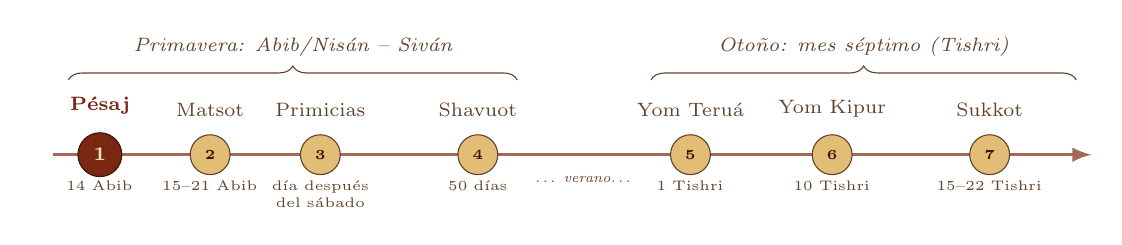
\begin{tikzpicture}[x=1cm,y=1cm,font=\scriptsize]
 \def\fiestaactual{1}
 \draw[line width=1.2pt,tierraroja!70,-{Latex[length=2.5mm]}] (0,0) -- (13.2,0);
 \draw[decorate,decoration={brace,amplitude=5pt},sepia] (0.2,0.95) -- (5.9,0.95) node[midway,above=5pt,font=\scriptsize\itshape]{Primavera: Abib/Nisán -- Siván};
 \draw[decorate,decoration={brace,amplitude=5pt},sepia] (7.6,0.95) -- (13.0,0.95) node[midway,above=5pt,font=\scriptsize\itshape]{Otoño: mes séptimo (Tishri)};
 \foreach \n/\x/\t/\d in {1/0.6/Pésaj/{14 Abib},2/2.0/Matsot/{15--21 Abib},3/3.4/Primicias/{día después del sábado},4/5.4/Shavuot/{50 días},5/8.1/Yom Teruá/{1 Tishri},6/9.9/Yom Kipur/{10 Tishri},7/11.9/Sukkot/{15--22 Tishri}}{
   \ifnum\n=\fiestaactual
     \node[circle,fill=tierraroja,draw=caferojizo,minimum size=5.5mm,text=papiro,font=\scriptsize\bfseries] at (\x,0) {\n};
     \node[above=3pt,font=\scriptsize\bfseries,text=tierraroja] at (\x,0.28) {\t};
   \else
     \node[circle,fill=mostaza!70,draw=sepia,minimum size=4.5mm,text=caferojizo,font=\tiny\bfseries] at (\x,0) {\n};
     \node[above=3pt,text=sepia] at (\x,0.25) {\t};
   \fi
   \node[below=6pt,text width=1.6cm,align=center,font=\tiny,text=sepia] at (\x,0) {\d};}
 \node[font=\tiny\itshape,text=sepia] at (6.75,-0.32) {\ldots\ verano\ldots};
\end{tikzpicture}\par
{\footnotesize\color{sepia}\textit{Figura 1.} El ciclo de Levítico 23; en rojo, la fiesta de este estudio. \textit{Nota.} Elaboración propia.}
\end{center}

Pésaj abre el año y también la primera semana festiva. En la Torá, la Pascua (día 14) y la fiesta de los Panes sin levadura (días 15 a 21) son dos solemnidades distintas aunque contiguas, y el Nuevo Testamento llega a nombrarlas juntas (``la fiesta de los panes sin levadura, que se llama la pascua'', Lc 22:1). Aquí nos ocupamos de la primera; la segunda tiene su propio capítulo en la serie.

%===================================================================
\section{El texto: la Pascua en la Torá y en la historia}

\subsection{Texto ancla: Éxodo 12:13}
El centro de la institución es una promesa que Dios hace a Moisés y Aarón ``en la tierra de Egipto'' (Éx 12:1), antes de que nada haya ocurrido:

\hebverso{וְהָיָה הַדָּם לָכֶם לְאֹת עַל הַבָּתִּים אֲשֶׁר אַתֶּם שָׁם \\ וְרָאִיתִי אֶת־הַדָּם וּפָסַחְתִּי עֲלֵכֶם \\ וְלֹא־יִהְיֶה בָכֶם נֶגֶף לְמַשְׁחִית בְּהַכֹּתִי בְּאֶרֶץ מִצְרָיִם}
\begin{cita}Y la sangre os será por señal en las casas donde vosotros estéis; y veré la sangre y pasaré de vosotros, y no habrá en vosotros plaga de mortandad cuando hiera la tierra de Egipto.\fuente{(Éx 12:13)}\end{cita}

El verso avanza en tres tiempos. La sangre es ``señal'' (\heb{אוֹת}, \emph{ot}) ``para vosotros'' (\heb{לָכֶם}); la marca está en la casa, pero el texto la orienta hacia quienes están dentro. Después Dios ``ve'' y ``pasa'' (\heb{וּפָסַחְתִּי}, \emph{ufasajtí}), el verbo que da nombre a la fiesta. Y de ahí la consecuencia: no habrá ``plaga'' (\heb{נֶגֶף}, \emph{néguef}) ``para destrucción'' (\heb{לְמַשְׁחִית}, \emph{lemashjit}). Sangre, mirada, paso, vida; la fiesta entera cabe en esa secuencia.

Los versos que rodean el texto ancla dan el procedimiento, con precisión de calendario y de cocina:

\begin{cita}Hablad a toda la congregación de Israel, diciendo: En el diez de este mes tómese cada uno un cordero según las familias de los padres, un cordero por familia\ldots{} El animal será sin defecto, macho de un año; lo tomaréis de las ovejas o de las cabras. Y lo guardaréis hasta el día catorce de este mes, y lo inmolará toda la congregación del pueblo de Israel entre las dos tardes.\fuente{(Éx 12:3, 5--6)}\end{cita}

\begin{cita}Y tomarán de la sangre, y la pondrán en los dos postes y en el dintel de las casas en que lo han de comer. Y aquella noche comerán la carne asada al fuego, y panes sin levadura; con hierbas amargas lo comerán\ldots{} Y lo comeréis así: ceñidos vuestros lomos, vuestro calzado en vuestros pies, y vuestro bordón en vuestra mano; y lo comeréis apresuradamente; es la Pascua de \SENOR.\fuente{(Éx 12:7--8, 11)}\end{cita}


\subsection{Todas las leyes de la Pascua}
La Torá vuelve a la Pascua en diez pasajes. Ninguno lo dice todo y cada uno añade algo; leídos juntos muestran cómo una instrucción dada para una noche en Egipto se convierte en institución para las generaciones siguientes, para el desierto, para la tierra y para el santuario central:

\begin{table}[!htbp]\centering\small\renewcommand{\arraystretch}{1.2}
\begin{tabular}{@{}L{2.3cm}L{3.3cm}L{8.8cm}@{}}
\toprule
\textbf{Texto} & \textbf{Contexto} & \textbf{Qué añade} \\ \midrule
Éx 12:1--14 & Egipto, antes de la décima plaga & Nuevo comienzo del año; cordero el 10, inmolado el 14 ``entre las dos tardes''; sangre en postes y dintel; asado, con \emph{matsot} y hierbas amargas; comido de prisa; ``memoria'' y ``estatuto perpetuo''. \\
Éx 12:21--28 & Moisés a los ancianos & Hisopo y lebrillo; nadie sale de casa hasta la mañana; el \emph{mashjit} no entra; la pregunta de los hijos: ``¿Qué es este rito vuestro?''. \\
Éx 12:43--51 & Después de la salida & Quién come: ningún extranjero incircunciso; el esclavo y el residente circuncidados, sí; ``una misma ley''; se come en una casa; ``ni quebraréis hueso suyo'' (12:46). \\
Éx 13:1--16 & Camino a Canaán & Consagración de los primogénitos y su rescate; \emph{matsot} siete días; ``lo contarás en aquel día a tu hijo'' (13:8); señal en la mano y memorial entre los ojos. \\
Éx 23:15--18 & Código de la alianza & Ázimos ``en el tiempo del mes de Abib''; no ofrecer con pan leudo la sangre del sacrificio; la grasa no queda hasta la mañana. \\
Éx 34:25 & Renovación del pacto & Nombra el ``sacrificio de la fiesta de la pascua'': nada leudado con su sangre, nada queda hasta la mañana. \\
Lv 23:5 & Reglamento de las solemnidades & Fecha y pertenencia: 14 del mes primero, ``entre las dos tardes'', ``pascua es de \SENOR''. \\
Nm 9:1--14 & Sinaí, segundo año & Primera Pascua del desierto; segunda Pascua (14 del mes segundo) para el impuro por muerto y el que está de viaje; castigo al que, pudiendo, no la hace; el extranjero puede celebrarla. \\
Nm 28:16 & Calendario de ofrendas & Fecha de la Pascua; las ofrendas del templo se prescriben para los siete días de Ázimos (28:17--25), no para el día 14. \\
Dt 16:1--8 & Discurso en Moab & ``Guardarás el mes de Abib''; ``de noche''; la Pascua ya no en las casas sino ``en el lugar que \SENOR{} escogiere''; ``ovejas y vacas''; ``a la puesta del sol''; verbo \emph{bashal} (16:7). \\
\bottomrule
\end{tabular}\par
{\footnotesize\color{sepia}\textit{Tabla 1.} Tabla sinóptica de las leyes de la Pascua. \textit{Nota.} Elaboración propia sobre la RVR1960 y la BHS.}
\end{table}

En la tabla se aprecian tres desplazamientos. La Pascua pasa de la \destacar{casa} al \destacar{santuario} (Dt 16:2, 6), de la \destacar{noche única} a la \destacar{memoria perpetua} (Éx 12:14, 17, 24), y de Israel a \destacar{quien se une a Israel}, pues el extranjero circuncidado ``será como uno de vuestra nación'' (Éx 12:48; Nm 9:14).

\subsection{La segunda Pascua: Números 9}
Números 9 registra un caso que Éxodo no había previsto. Algunos hombres estaban impuros por haber tocado un cadáver y no podían celebrar la Pascua en su fecha. Se presentan ante Moisés y preguntan por qué se les impide presentar la ofrenda del \SENOR{} a su tiempo, junto con los demás (Nm 9:7, paráfrasis). Moisés no improvisa una respuesta: ``Esperad, y oiré lo que ordena \SENOR{} acerca de vosotros'' (9:8). Lo que Dios ordena es una segunda fecha:

\begin{cita}Cualquiera de vosotros o de vuestros descendientes, que estuviere inmundo por causa de muerto o estuviere de viaje lejos, celebrará la pascua a \SENOR. En el mes segundo, a los catorce días del mes, entre las dos tardes, la celebrarán; con panes sin levadura y hierbas amargas la comerán.\fuente{(Nm 9:10--11)}\end{cita}

La tradición la llamó \emph{Pésaj Shení}, ``segunda Pascua''. Del texto se desprenden tres cosas. La fecha importa, porque la que se fija es también un día 14 ``entre las dos tardes'' y no un día cualquiera. La exclusión del impuro no es definitiva, porque Dios abre un camino para quien no pudo llegar. Y quien, estando limpio y sin viaje, deja de celebrarla ``será cortado de entre su pueblo'' (9:13), de modo que la Pascua no es opcional para el que pertenece a Israel. El mismo capítulo repite una norma de Éxodo (``ni quebrarán hueso de él'', 9:12) y extiende la fiesta al extranjero (9:14). Ezequías apelará a este precedente (2~Cr 30:2--3, 15).

\subsection{Deuteronomio 16: el lugar escogido y el verbo \emph{bashal}}
Deuteronomio reformula la Pascua para la vida en la tierra. Ya no hay sangre en las puertas; el sacrificio se hace en el santuario y la familia vuelve después ``a sus tiendas''.

\hebverso{וּבִשַּׁלְתָּ וְאָכַלְתָּ בַּמָּקוֹם אֲשֶׁר יִבְחַר יְהוָה אֱלֹהֶיךָ בּוֹ \\ וּפָנִיתָ בַבֹּקֶר וְהָלַכְתָּ לְאֹהָלֶיךָ}
\begin{cita}Y la asarás y comerás en el lugar que \SENOR{} tu Dios hubiere escogido; y por la mañana regresarás y volverás a tu habitación.\fuente{(Dt 16:7)}\end{cita}

La RVR1960 traduce ``la asarás''. El hebreo dice \heb{וּבִשַּׁלְתָּ} (\emph{uvishaltá}), del verbo \heb{בָּשַׁל} (\emph{bashal}), que normalmente significa ``cocer, hervir'', y eso es justamente lo que Éxodo 12:9 había prohibido: ``Ninguna cosa comeréis de él cruda, ni cocida en agua (\heb{וּבָשֵׁל מְבֻשָּׁל בַּמָּיִם}), sino asada al fuego''. Deuteronomio permite además \emph{tson uvakar}, ``ovejas y vacas'' (16:2), donde Éxodo exigía un \emph{seh} de ovejas o cabras.

\begin{nota}[Precisión: una tensión que la Biblia misma armoniza]
La diferencia entre Éx 12:9 y Dt 16:7 se explica de varias maneras. (1) \emph{Bashal} tiene un sentido amplio, ``cocinar, preparar al fuego'', y no solo ``hervir''; Éx 12:9 lo precisa con ``en agua'' porque sin ese complemento podría designar también el asado (así Tigay, 1996, y la exégesis judía tradicional). (2) Deuteronomio refleja otra etapa de la práctica, centralizada en el santuario. (3) Las ``vacas'' de 16:2 se refieren a las ofrendas festivas de la semana, no al animal pascual (lectura rabínica). El cronista ya armoniza los dos textos en la Pascua de Josías: \heb{וַיְבַשְּׁלוּ הַפֶּסַח בָּאֵשׁ כַּמִּשְׁפָּט}, ``y asaron la pascua al fuego conforme a la ordenanza; mas lo que había sido santificado lo cocieron en ollas, en calderos y en sartenes'' (2~Cr 35:13). Usa el verbo de Deuteronomio (\emph{bashal}) con el complemento de Éxodo (``al fuego''), y distingue el cordero de las demás ofrendas. La Biblia interpreta la Biblia dentro de su propio canon.
\end{nota}

El otro dato de Deuteronomio es la hora. La Pascua se sacrifica ``por la tarde a la puesta del sol'' (\heb{בָּעֶרֶב כְּבוֹא הַשֶּׁמֶשׁ}), en el tiempo señalado (\emph{moed}) de la salida de Egipto (Dt 16:6, paráfrasis); el momento del sacrificio queda unido a la hora del éxodo. Volveremos sobre esta hora al estudiar \emph{bein ha'arbayim}.

%===================================================================
\section{Lectura histórica}

\subsection{Abib: la fiesta en el calendario de la cebada}
El mes de la Pascua se llama en la Torá \heb{חֹדֶשׁ הָאָבִיב} (\emph{jódesh ha'aviv}, Éx 13:4; 23:15; 34:18; Dt 16:1). En origen \emph{aviv} no nombra un mes sino un estado del grano: la cebada ``espigada'', con la espiga ya formada y todavía verde. Así lo usa el relato de las plagas: ``el lino, pues, y la cebada fueron destrozados, porque la cebada estaba ya espigada (\heb{אָבִיב}), y el lino en caña'' (Éx 9:31). La Pascua cae, por tanto, a fines de marzo o en abril, cuando la cebada madura en Egipto y en la tierra de Israel, después de las lluvias de invierno y antes de la siega del trigo. El nombre babilonio \emph{Nisán}, que se impuso después del exilio, aparece en Neh 2:1 y Est 3:7.

El calendario bíblico es lunar con ajuste solar. El mes empieza con la luna nueva, de modo que el día 14 coincide con la luna llena y la noche de la Pascua es una noche clara. Para que el ``mes de Abib'' siga siendo el de las espigas hace falta un ajuste con las estaciones (un mes adicional en algunos años, el posterior \emph{Adar Shení} o \emph{Veadar}); la Torá no describe ese mecanismo, lo supone.

\begin{nota}[Precisión]
El calendario judío calculado y la regla del mes intercalar son rabínicos (siglos \textsc{iv}--\textsc{x} e.\,c.); la observación de la cebada que defienden los caraítas se apoya en el sentido de \emph{aviv}, pero tampoco está prescrita. Lo explícito es que la Pascua pertenece al mes de las espigas y que el día 14 es luna llena.
\end{nota}

\subsection{Egipto del Nuevo Reino y la fecha del éxodo}
El relato sitúa a Israel en el delta oriental del Nilo, en la tierra de Gosén, trabajando en las ciudades de almacenamiento ``Pitón y Ramesés'' (Éx 1:11). Ramesés corresponde a \emph{Pi-Ramsés}, la capital del delta en tiempos de Ramsés II (siglo \textsc{xiii} a.\,e.\,c.), identificada con Qantir y la vecina Tell el-Dab'a (la antigua Avaris). Sobre este dato, entre otros, se apoya la llamada fecha tardía del éxodo, hacia 1260 a.\,e.\,c. (Hoffmeier, 1997). La cronología interna de 1~R 6:1 (480 años entre la salida y el cuarto año de Salomón) lleva en cambio a una fecha temprana, hacia 1446 a.\,e.\,c., en tiempos de la dinastía XVIII.

\begin{nota}[Precisión: la fecha del éxodo]
La serie fecha la salida de Egipto en 1529--1530 a.\,e.\,c. La cronología de 1~R 6:1 (480 años antes del cuarto año de Salomón, ca.\ 966 a.\,e.\,c.) da ca.\ 1446 a.\,e.\,c.; muchos historiadores, apoyados en el nombre ``Ramesés'' de Éx 1:11 y en la arqueología del delta, proponen ca.\ 1260 a.\,e.\,c. Las tres fechas dependen de cómo se lean los números bíblicos (literales o generacionales) y de la sincronía con Egipto. El texto bíblico no da una fecha absoluta, y ninguna de estas cifras altera el contenido teológico de la Pascua.
\end{nota}

\subsection{``Contra todos los dioses de Egipto''}
Éxodo 12:12 interpreta la décima plaga como un juicio religioso: \heb{וּבְכָל־אֱלֹהֵי מִצְרַיִם אֶעֱשֶׂה שְׁפָטִים אֲנִי יְהוָה}, ``y ejecutaré mis juicios en todos los dioses de Egipto. Yo \SENOR''. Números lo repite al recordar la salida: mientras los egipcios enterraban a sus primogénitos, ``también había hecho \SENOR{} juicios contra sus dioses'' (Nm 33:4). El conflicto, pues, va más allá de lo político y alcanza la pretensión divina de Egipto. En la ideología egipcia el faraón era hijo del dios sol y garante del orden cósmico (\emph{maat}), y su primogénito heredaba esa función; la muerte del primogénito del faraón ``que se sentaba sobre su trono'' (Éx 12:29) golpea el centro de ese sistema.

\begin{nota}[Precisión]
Es frecuente asignar cada plaga a un dios egipcio concreto (el Nilo a Hapi, las ranas a Heqet, las tinieblas a Ra, etc.). Algunas correspondencias son razonables (el Nilo, el sol), otras son forzadas. El texto bíblico solo afirma el juicio ``contra todos los dioses'' en relación con la décima plaga (Éx 12:12; Nm 33:4) y, de modo general, que las plagas muestran que ``no hay otro como yo en toda la tierra'' (Éx 9:14). No parece prudente construir una teología sobre una tabla de correspondencias que el texto no da (cf.\ Sarna, 1991; Hoffmeier, 1997).
\end{nota}

\subsection{Los primogénitos: ``Israel es mi hijo''}
La décima plaga fue anunciada mucho antes de la Pascua, en las primeras palabras que Dios pone en boca de Moisés frente al faraón:

\begin{cita}Y dirás a Faraón: \SENOR{} ha dicho así: Israel es mi hijo, mi primogénito. Ya te he dicho que dejes ir a mi hijo, para que me sirva, mas no has querido dejarlo ir; he aquí yo voy a matar a tu hijo, tu primogénito.\fuente{(Éx 4:22--23)}\end{cita}

La lógica es de correspondencia: el faraón retiene al primogénito de Dios y Dios reclama al primogénito del faraón. Pero la noche de la Pascua el juicio no distingue por etnia sino por la sangre, y el primogénito israelita que estuviera en una casa sin marcar no tenía protección. Por eso, apenas salido de Egipto, Dios reclama a los primogénitos de Israel como suyos: ``Conságrame todo primogénito\ldots{} mío es'' (Éx 13:2). Los que fueron salvados quedan rescatados y dedicados; el padre debe ``redimir'' a su hijo primogénito (Éx 13:13--15), y más tarde los levitas toman el lugar de los primogénitos, porque desde el día en que Dios hirió a los primogénitos de Egipto los santificó para sí (Nm 3:13, paráfrasis). De la Pascua nace así una teología de la pertenencia: el que fue librado de la muerte ya no se pertenece.

\subsection{Del 10 al 15 de Abib: la cronología de Éxodo 12}
Éxodo 12 fija una secuencia de días que la Pascua repetirá cada año. El animal se escoge el día 10 y se ``guarda'' (\heb{לְמִשְׁמֶרֶת}, \emph{lemishméret}) hasta el 14; se inmola ``entre las dos tardes'' de ese día y se come esa noche; a medianoche mueren los primogénitos (12:29), e Israel sale el 15, ``el segundo día de la pascua'' (Nm 33:3).

\begin{figure}[!htbp]\centering
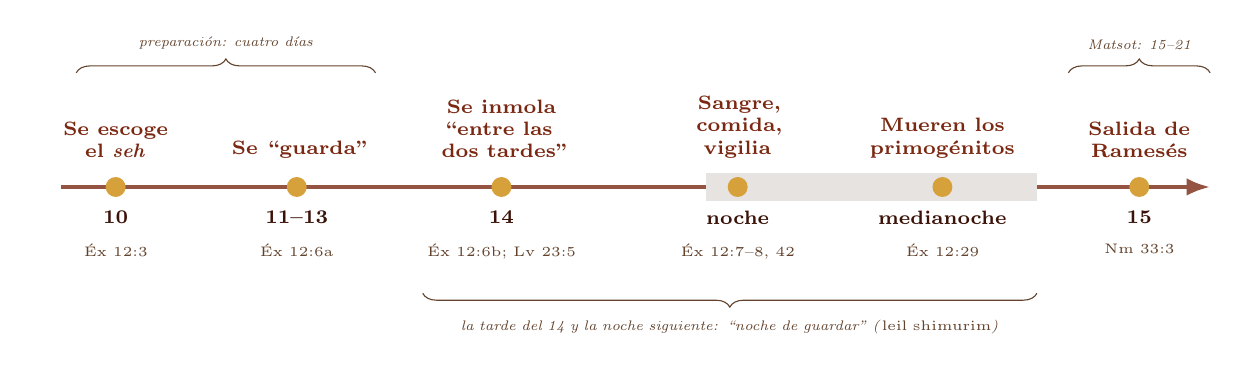
\begin{tikzpicture}[x=1cm,y=1cm,font=\scriptsize]
 \draw[line width=1.4pt,tierraroja!80,-{Latex[length=3mm]}] (0,0) -- (14.6,0);
 \fill[caferojizo!12] (8.2,-0.18) rectangle (12.4,0.18);
 \foreach \x/\d/\t/\r in {0.7/10/{Se escoge el \emph{seh}}/{Éx 12:3}, 3.0/{11--13}/{Se ``guarda''}/{Éx 12:6a}, 5.6/14/{Se inmola ``entre las dos tardes''}/{Éx 12:6b; Lv 23:5}, 8.6/{noche}/{Sangre, comida, vigilia}/{Éx 12:7--8, 42}, 11.2/{medianoche}/{Mueren los primogénitos}/{Éx 12:29}, 13.7/15/{Salida de Ramesés}/{Nm 33:3}}{
   \fill[mostaza] (\x,0) circle (3.6pt);
   \node[above=7pt,text width=2.0cm,align=center,font=\scriptsize\bfseries,text=tierraroja] at (\x,0) {\t};
   \node[below=5pt,font=\scriptsize\bfseries,text=caferojizo] at (\x,0) {\d};
   \node[below=17pt,text width=2.0cm,align=center,font=\tiny,text=sepia] at (\x,0) {\r};}
 \draw[decorate,decoration={brace,amplitude=5pt,mirror},sepia] (4.6,-1.35) -- (12.4,-1.35) node[midway,below=6pt,font=\tiny\itshape,text=sepia,text width=8cm,align=center]{la tarde del 14 y la noche siguiente: ``noche de guardar'' (\emph{leil shimurim})};
 \draw[decorate,decoration={brace,amplitude=5pt},sepia] (0.2,1.45) -- (4.0,1.45) node[midway,above=5pt,font=\tiny\itshape,text=sepia]{preparación: cuatro días};
 \draw[decorate,decoration={brace,amplitude=5pt},sepia] (12.8,1.45) -- (14.6,1.45) node[midway,above=5pt,font=\tiny\itshape,text=sepia]{Matsot: 15--21};
\end{tikzpicture}\par
{\footnotesize\color{sepia}\textit{Figura 2.} Del 10 al 15 de Abib en Éxodo 12. \textit{Nota.} Elaboración propia. Si la noche de la comida pertenece todavía al 14 o ya al 15 se discute en la sección 5.3.}
\end{figure}

La noche tiene nombre propio. Después de la salida, el narrador la define: \heb{לֵיל שִׁמֻּרִים הוּא לַיהוָה}, ``es noche de guardar para \SENOR, por haberlos sacado en ella de la tierra de Egipto. Esta noche deben guardarla para \SENOR{} todos los hijos de Israel en sus generaciones'' (Éx 12:42). La palabra \emph{shimurim} aparece solo aquí, dos veces en el mismo versículo (conteo propio sobre el Códice de Leningrado), y el doble uso no parece casual: es la noche en que \emph{Dios} veló sobre Israel, y por eso la noche en que \emph{Israel} vela para Dios.

\subsection{Ramesés y Sucot: el primer tramo}
``Partieron los hijos de Israel de Ramesés a Sucot, como seiscientos mil hombres de a pie, sin contar los niños'' (Éx 12:37). Números 33:3--7 da el itinerario oficial: Ramesés, Sucot, Etam ``al confín del desierto'', y luego el giro hacia Pi-hahirot, frente a Baal-zefón, delante de Migdol. Las dos primeras etapas tienen identificaciones razonables, las demás siguen en discusión. Sucot suele identificarse con la región de Tjeku, en el Uadi Tumilat, y en particular con Tell el-Maskhuta; Pitón, con Tell er-Retaba o con la misma Maskhuta (Hoffmeier, 1997).

\begin{figure}[!htbp]\centering
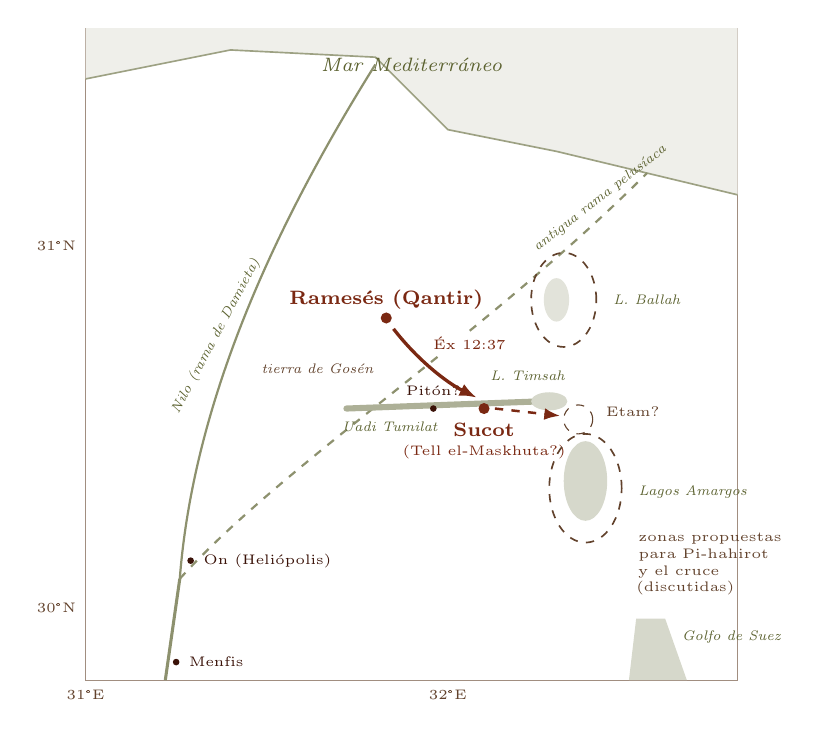
\begin{tikzpicture}[x=4.6cm,y=4.6cm,font=\scriptsize]
 \draw[sepia!60,line width=0.4pt] (0,0) rectangle (1.8,1.8);
 \fill[oliva!10] (0,1.66) -- (0.4,1.74) -- (0.8,1.72) -- (1.0,1.52) -- (1.3,1.46) -- (1.8,1.34) -- (1.8,1.8) -- (0,1.8) -- cycle;
 \draw[oliva!60,line width=0.6pt] (0,1.66) -- (0.4,1.74) -- (0.8,1.72) -- (1.0,1.52) -- (1.3,1.46) -- (1.8,1.34);
 \node[font=\scriptsize\itshape,text=oliva] at (0.9,1.70) {Mar Mediterráneo};
 \draw[oliva!70,line width=1.1pt] (0.22,0.0) -- (0.26,0.28);
 \draw[oliva!70,line width=0.8pt] (0.26,0.28) .. controls (0.30,0.8) and (0.55,1.3) .. (0.80,1.70);
 \draw[oliva!70,line width=0.8pt,dashed] (0.26,0.28) .. controls (0.55,0.6) and (1.1,0.95) .. (1.55,1.40);
 \node[font=\tiny\itshape,text=oliva,rotate=62] at (0.36,0.95) {Nilo (rama de Damieta)};
 \node[font=\tiny\itshape,text=oliva,rotate=38] at (1.42,1.33) {antigua rama pelusíaca};
 \draw[oliva!50,line width=2.2pt,line cap=round] (0.72,0.75) -- (1.26,0.77);
 \node[font=\tiny\itshape,text=oliva] at (0.84,0.70) {Uadi Tumilat};
 \fill[oliva!25] (1.28,0.77) ellipse (0.05 and 0.025);
 \node[font=\tiny\itshape,text=oliva,anchor=south] at (1.22,0.80) {L.\ Timsah};
 \fill[oliva!25] (1.38,0.55) ellipse (0.06 and 0.11);
 \node[font=\tiny\itshape,text=oliva,anchor=west] at (1.50,0.52) {Lagos Amargos};
 \fill[oliva!25] (1.52,0.17) -- (1.60,0.17) -- (1.66,0.0) -- (1.50,0.0) -- cycle;
 \node[font=\tiny\itshape,text=oliva,anchor=west] at (1.62,0.12) {Golfo de Suez};
 \fill[oliva!18] (1.30,1.05) ellipse (0.035 and 0.06);
 \node[font=\tiny\itshape,text=oliva,anchor=west] at (1.43,1.05) {L.\ Ballah};
 \node[font=\tiny\itshape,text=sepia,fill=white,inner sep=1pt] at (0.64,0.86) {tierra de Gosén};
 \fill[caferojizo] (0.25,0.05) circle (1.2pt) node[anchor=west,font=\tiny,text=caferojizo] {\,Menfis};
 \fill[caferojizo] (0.29,0.33) circle (1.2pt) node[anchor=west,font=\tiny,text=caferojizo] {\,On (Heliópolis)};
 \fill[tierraroja] (0.83,1.00) circle (2pt) node[anchor=south,font=\scriptsize\bfseries,text=tierraroja,yshift=2pt,fill=white,inner sep=1pt] {Ramesés (Qantir)};
 \fill[tierraroja] (1.10,0.75) circle (2pt);
 \node[anchor=north,font=\scriptsize\bfseries,text=tierraroja,align=center,inner sep=1pt] at (1.10,0.72) {Sucot\\[-1pt]{\tiny\mdseries (Tell el-Maskhuta?)}};
 \fill[caferojizo] (0.96,0.75) circle (1.2pt) node[anchor=south,font=\tiny,text=caferojizo,yshift=1pt] {Pitón?};
 \draw[tierraroja,line width=1.2pt,-{Latex[length=2.2mm]}] (0.85,0.97) .. controls (0.92,0.88) and (1.0,0.82) .. (1.08,0.78);
 \node[font=\tiny,text=tierraroja,fill=white,inner sep=1pt] at (1.06,0.93) {Éx 12:37};
 \draw[tierraroja,line width=0.9pt,dashed,-{Latex[length=2mm]}] (1.13,0.75) -- (1.31,0.73);
 \draw[sepia,dashed] (1.36,0.72) circle (0.04);
 \node[font=\tiny,text=sepia,anchor=west] at (1.41,0.74) {Etam?};
 \draw[sepia,dashed,line width=0.6pt] (1.38,0.53) ellipse (0.10 and 0.15);
 \draw[sepia,dashed,line width=0.6pt] (1.32,1.05) ellipse (0.09 and 0.13);
 \node[font=\tiny,text=sepia,text width=2.0cm,align=left,anchor=west] at (1.50,0.32) {zonas propuestas para Pi-hahirot y el cruce (discutidas)};
 \foreach \l/\t in {0/31°E,1/32°E} {\node[below,font=\tiny,text=sepia] at (\l,0) {\t};}
 \foreach \l/\t in {0.2/30°N,1.2/31°N} {\node[left,font=\tiny,text=sepia] at (0,\l) {\t};}
\end{tikzpicture}\par
{\footnotesize\color{sepia}\textit{Figura 3.} Mapa esquemático del delta oriental: de Ramesés a Sucot. \textit{Nota.} Elaboración propia; coordenadas aproximadas reales de los sitios (Qantir 30,8°N 31,8°E; Tell el-Maskhuta 30,55°N 32,1°E). Las identificaciones con signo de interrogación y las zonas punteadas son discutidas.}
\end{figure}

La serie sigue a Números 33 para fechar las primeras jornadas: el 15 de Abib Israel se reúne en Sucot, el 16 va a Etam, el 17 llega frente al mar, donde el faraón lo alcanza. De esas fechas, la única firme es la primera: la salida fue el día 15, a la vista de los egipcios que sepultaban a sus primogénitos (Nm 33:3--4). Las demás son cálculos sobre el número de campamentos, y la serie los usa para su lectura de las Primicias (véase el estudio correspondiente).

\subsection{Las pascuas de la historia de Israel}
La Biblia recuerda pocas celebraciones concretas de la Pascua, y casi siempre en momentos de fundación o de restauración. El silencio entre una y otra pesa: 2~R 23:22 afirma que ``no había sido hecha tal pascua desde los tiempos en que los jueces gobernaban a Israel''.

\begin{table}[!htbp]\centering\small\renewcommand{\arraystretch}{1.2}
\begin{tabular}{@{}L{2.5cm}L{2.9cm}L{9.0cm}@{}}
\toprule
\textbf{Texto} & \textbf{Ocasión} & \textbf{Rasgos} \\ \midrule
Jos 5:10--12 & Gilgal, al entrar & Pascua el 14 ``por la tarde, en los llanos de Jericó'', después de la circuncisión de la nueva generación (5:2--9); al otro día, panes sin levadura y espigas tostadas del fruto de la tierra; ``el maná cesó''. \\
2~Cr 30 & Ezequías & Pascua en el mes segundo (precedente de Nm 9), porque los sacerdotes no estaban santificados y el pueblo no se había reunido; invitación a Efraín y Manasés; muchos comen impuros y Ezequías intercede (30:18--20); se prolonga siete días más. \\
2~R 23:21--23; 2~Cr 35:1--19 & Josías, año 18 & Pascua ``conforme a lo que está escrito en el libro de este pacto''; centralizada en Jerusalén; levitas que degüellan, sacerdotes que rocían la sangre (35:11); el rey aporta 30\,000 corderos y cabritos (35:7). \\
Esd 6:19--22 & Regreso del exilio, 515 a.\,e.\,c. & Tras la dedicación del segundo templo; sacerdotes y levitas purificados; comen los repatriados y quienes se habían apartado de la impureza de las naciones. \\
Ez 45:21--24 & Visión del templo futuro & ``Tendréis la pascua, fiesta de siete días''; el príncipe ofrece un becerro ``por el pecado'' por sí y por el pueblo (45:22). \\
\bottomrule
\end{tabular}\par
{\footnotesize\color{sepia}\textit{Tabla 2.} Las pascuas narradas en la Biblia hebrea. \textit{Nota.} Elaboración propia sobre la RVR1960.}
\end{table}

Estas pascuas siguen un patrón: cada nueva etapa de Israel empieza con una. En Gilgal, la generación nacida en el desierto es circuncidada, celebra la Pascua, come del fruto de la tierra y el maná cesa; la fiesta de salida se ha vuelto fiesta de entrada. Ezequías y Josías la convierten en acto de reforma, y Ezequías ora por los que comieron sin estar purificados: ``oyó \SENOR{} a Ezequías, y sanó al pueblo'' (2~Cr 30:20). Esdras la celebra al terminar el segundo templo, y Ezequiel la proyecta al templo de la restauración, con un \emph{jatat} del príncipe el día 14 (Ez 45:22), dato que retomaremos en la sección 10.2.


\subsection{La Pascua en el Segundo Templo}
En tiempos de Jesús la Pascua era la fiesta de peregrinación más concurrida. Los corderos se degollaban en los atrios del templo la tarde del 14 y se comían por grupos (\emph{javurot}) dentro de los límites de Jerusalén. Las fuentes de la época dan detalles valiosos, cada una desde su perspectiva:

\begin{itemize}\setlength{\itemsep}{2pt}
\item \textbf{Josefo} explica el nombre (\grc{πάσχα}, que, dice, significa \grc{ὑπερβάσια}, ``paso por encima''; \emph{Antigüedades} 2.313) y narra que, antes de la guerra, el gobernador Cestio pidió a los sacerdotes contar las víctimas pascuales: según su relato se degollaron unas 255\,600 (la cifra varía en los manuscritos) entre la hora novena y la undécima, aproximadamente entre las 15 y las 17 horas, con no menos de diez comensales por víctima (\emph{Guerra} 6.423--427). La cifra es de Josefo y probablemente está inflada; lo que sí vale es el dato de la hora y del grupo mínimo.
\item \textbf{Filón} de Alejandría llama a la Pascua \grc{διαβατήρια}, ``fiesta del cruce'', y subraya que ese día todo el pueblo actúa como sacerdote, porque cada uno inmola su propia víctima (\emph{De specialibus legibus} 2.145--146).
\item \textbf{El papiro pascual de Elefantina} (419 a.\,e.\,c.) instruye a la colonia judía de Egipto sobre la pureza y los panes sin levadura del 15 al 21 de Nisán; la palabra ``pascua'' es allí una restitución (Porten \& Yardeni, 1986, A4.1).
\item \textbf{La Misná} (ca.\ 200 e.\,c.) recuerda en el tratado \emph{Pesajim} que el cordero se sacrificaba después del sacrificio vespertino, que el pueblo entraba en tres turnos (\emph{kitot}), que los levitas cantaban el \emph{Hallel} (Sal 113--118) mientras se degollaba, y que los sacerdotes pasaban la sangre en vasijas de oro y plata hasta el altar (m.~Pesajim 5:1--10).
\end{itemize}

\begin{nota}[Precisión: fuentes posteriores]
La Misná se redactó más de un siglo después de la destrucción del templo (70 e.\,c.) y describe el culto con rasgos idealizados; sus datos coinciden en parte con Josefo y con 2~Cr 35, pero no deben leerse como acta notarial. El \emph{séder} familiar con cuatro copas, preguntas fijas y \emph{Hagadá} (m.~Pesajim 10) es, según Bokser (1984), un desarrollo rabínico posterior al 70 e.\,c., que reemplazó al sacrificio por una comida de estudio y memoria con forma de banquete grecorromano. La última cena de Jesús es anterior a esa forma, aunque compartía con ella elementos (pan, copa, bendiciones, himno).
\end{nota}

%===================================================================
\section{Lectura filológica}

El vocabulario de Éxodo 12 es concreto (una puerta, un animal, una hora, una hierba, un verbo de movimiento), y cada palabra conserva una escena. Varias de ellas pasan al griego y al Nuevo Testamento con su carga intacta.

\subsection{El nombre de la fiesta}

\begin{filologia}[\heb{פֶּסַח} \emph{pésaj}]
\textbf{Raíz} \heb{פ־ס־ח} (\emph{p-s-j}). El sustantivo \emph{pésaj} aparece 49 veces en 46 versículos de la Biblia hebrea (conteo propio del lema, Strong H6453, sobre el Códice de Leningrado; el verbo \emph{pasaj}, H6452, suma otras ocho) y designa a la vez la fiesta, el animal (``sacrificad la pascua'', Éx 12:21) y el sacrificio (\heb{זֶבַח־פֶּסַח}, ``la víctima de la pascua'', 12:27). El verbo da tres familias de sentido:\par\smallskip
\begin{tabular}{@{}L{3.4cm}L{11.0cm}@{}}
\emph{pasar por encima, saltar} & \heb{וּפָסַחְתִּי עֲלֵכֶם} ``pasaré de vosotros'' (Éx 12:13); \heb{וּפָסַח יְהוָה עַל־הַפֶּתַח} ``pasará \SENOR{} aquella puerta'' (12:23); ``pasó por encima de las casas'' (12:27). En 1~R 18:26 el piel \heb{וַיְפַסְּחוּ} describe a los profetas de Baal que ``saltaban'' (o danzaban cojeando) alrededor del altar. \\[2pt]
\emph{cojear, vacilar} & \heb{פֹּסְחִים עַל־שְׁתֵּי הַסְּעִפִּים} ``¿hasta cuándo claudicaréis entre dos pensamientos?'' (1~R 18:21); el adjetivo \heb{פִּסֵּחַ} \emph{piséaj}, ``cojo'' (Lv 21:18; 2~S 9:13); Mefi-boset ``quedó cojo'' (\heb{וַיִּפָּסֵחַ}, 2~S 4:4). \\[2pt]
\emph{proteger, amparar} & \heb{גָּנוֹן וְהִצִּיל פָּסֹחַ וְהִמְלִיט} ``amparando, librando, preservando y salvando'' (Is 31:5): \emph{pasoaj} en paralelo con verbos de defensa, en una imagen de aves que revolotean sobre el nido. \\
\end{tabular}\par\smallskip
\textbf{Lecturas antiguas.} La LXX traduce Éx 12:13 y 12:27 con \grc{σκεπάζω}, ``cubrir, proteger'' (\grc{σκεπάσω ὑμᾶς}), y 12:23 con \grc{παρελεύσεται}, ``pasará de largo''. El Targum Onqelos traduce ``tendré piedad''. Rashi registra las dos opciones: \emph{ufasajtí} es ``tendré compasión'', como en Is 31:5, ``y yo digo: todo \emph{pesijá} es lenguaje de salto y brinco'' (Rashi a Éx 12:13). Josefo (\grc{ὑπερβάσια}) y Filón (\grc{διαβατήρια}) toman el sentido de paso.
\end{filologia}

Los dos sentidos no se excluyen. La imagen de 12:23 es espacial: Dios recorre Egipto ``para herir'' (\heb{לִנְגֹּף}), llega a una puerta marcada y la ``salta'' sin entrar, y ``no dejará entrar al heridor en vuestras casas''. La de Is 31:5 es de protección activa, porque el ave que se cierne sobre su nido no pasa de largo, se queda encima. Traducir ``pasar de largo'' destaca el juicio que no toca; traducir ``proteger'' destaca la presencia que guarda. El texto de Éxodo pide ambas cosas, porque el mismo \SENOR{} que pasa por Egipto es quien impide la entrada del \emph{mashjit}.

\begin{filologia}[\heb{בֵּין הָעַרְבָּיִם} \emph{bein ha'arbayim}]
Literalmente ``entre las dos tardes'' (dual de \heb{עֶרֶב}, \emph{érev}). Fija la hora del sacrificio pascual (Éx 12:6; Lv 23:5; Nm 9:3, 5, 11) y también la del sacrificio vespertino diario (Éx 29:39, 41), la de encender las lámparas (Éx 30:8) y la de la llegada de las codornices (Éx 16:12). Se interpretó de tres maneras:\par\smallskip
\begin{tabular}{@{}L{3.6cm}L{10.8cm}@{}}
\emph{Desde el declinar del sol hasta la puesta} & Primera ``tarde'' cuando el sol comienza a bajar (después del mediodía), segunda ``tarde'' al ponerse. Es la práctica del Segundo Templo: Josefo, entre la hora 9 y la 11 (\emph{Guerra} 6.423); la Misná, después del \emph{tamid} vespertino, hacia las 8½ horas (m.~Pesajim 5:1). Fariseos y rabinos; Rashi a Éx 12:6. \\[2pt]
\emph{Entre la puesta y la oscuridad} & Primera ``tarde'' la puesta del sol, segunda la caída de la noche. Samaritanos, caraítas, Ibn Ezra a Éx 12:6. Se apoya en Dt 16:6, ``a la puesta del sol''. \\[2pt]
\emph{Al comenzar el día 14} & Variante de la segunda: el sacrificio al anochecer con que \emph{empieza} el 14 y la comida esa misma noche. Es la práctica de la serie. \\
\end{tabular}
\end{filologia}

\subsection{El animal y la sangre}

\begin{filologia}[\heb{שֶׂה תָמִים} \emph{seh tamim}]
\heb{שֶׂה} (\emph{seh}) no es ``cordero'' en sentido estricto, sino una cabeza de ganado menor, oveja o cabra: ``lo tomaréis de las ovejas o de las cabras'' (\heb{מִן־הַכְּבָשִׂים וּמִן־הָעִזִּים}, Éx 12:5). La RVR1960 traduce ``cordero'' en 12:3--4 y ``el animal'' en 12:5. \heb{תָּמִים} (\emph{tamim}), ``íntegro, completo, sin defecto'', es el adjetivo de los animales aptos para el altar (Lv 22:19--21) y también de Noé (Gn 6:9) y de Abraham (``sé perfecto'', Gn 17:1). Se exige además \heb{זָכָר בֶּן־שָׁנָה} (\emph{zajar ben-shaná}), ``macho de un año''. La LXX traduce \grc{πρόβατον τέλειον}; 1~P 1:19 hablará del ``cordero sin mancha y sin contaminación'' (\grc{ἀμνοῦ ἀμώμου καὶ ἀσπίλου}).
\end{filologia}

\begin{filologia}[\heb{דָּם} \emph{dam} y \heb{אוֹת} \emph{ot}]
\heb{דָּם} (\emph{dam}), ``sangre'', aparece seis veces en Éx 12:7--23 (vv. 7, 13 [2×], 22 [2×], 23; conteo propio sobre el Códice de Leningrado). La ley posterior fundará su valor en Lv 17:11: ``la vida de la carne en la sangre está''. En Éxodo 12, sin embargo, la sangre no se lleva a un altar: se pone en la puerta. Su función es ser \heb{אוֹת} (\emph{ot}), ``señal'', la misma palabra del arco iris (Gn 9:12--13), de la circuncisión (Gn 17:11) y del sábado (Éx 31:13). La señal es \heb{לָכֶם}, ``para vosotros'' (12:13); Rashi comenta: ``para vosotros por señal, y no para otros''. A la vez, el texto dice que Dios ``ve'' la sangre (12:13, 23): la señal está ante los ojos de Dios y ante la conciencia de la familia.
\end{filologia}

\begin{filologia}[\heb{הַמַּשְׁחִית} \emph{hamashjit}]
Participio hifil de \heb{שָׁחַת} (\emph{shajat}), ``arruinar, destruir'': ``el destructor''. En Éx 12:13 la forma \heb{לְמַשְׁחִית} se traduce ``de mortandad'' (``plaga para destrucción''); en 12:23 tiene artículo y es un agente: ``no dejará entrar al heridor (\heb{הַמַּשְׁחִית}) en vuestras casas''. El mismo término designa al ángel que hiere a Jerusalén en tiempos de David (2~S 24:16) y al ejército asolador (Jer 22:7, verbo). Hebreos 11:28 lo llama \grc{ὁ ὀλοθρεύων}, ``el que destruía a los primogénitos'', y 1~Co 10:10 \grc{ὁ ὀλοθρευτής}, ``el destructor''. El texto deja abierta la relación entre \SENOR{} que hiere (12:12, 29) y el \emph{mashjit}, que obra bajo su control.
\end{filologia}

\subsection{La puerta}

\begin{filologia}[\heb{מְזוּזֹת} \emph{mezuzot}, \heb{מַשְׁקוֹף} \emph{mashqof}, \heb{סַף} \emph{saf}, \heb{אֵזוֹב} \emph{ezov}]
\heb{שְׁתֵּי הַמְּזוּזֹת} (\emph{shtei hamezuzot}), ``los dos postes'' de la puerta; es la palabra que Dt 6:9 usa para escribir las palabras de Dios ``en los postes de tu casa'', y de ella viene la \emph{mezuzá} judía. \heb{מַשְׁקוֹף} (\emph{mashqof}), ``dintel'', la viga superior; aparece solo en Éx 12:7, 22, 23 (conteo propio sobre el Códice de Leningrado). \heb{סַף} (\emph{saf}) en 12:22 puede ser ``lebrillo'' (así la RVR1960) o ``umbral'' (sentido frecuente, p.\,ej.\ Jue 19:27); la LXX entiende \grc{παρὰ τὴν θύραν}, ``junto a la puerta''. \heb{אֵזוֹב} (\emph{ezov}), ``hisopo'', planta aromática de ramas finas usada para rociar (Lv 14:4; Nm 19:18; Sal 51:7 [51:9]); reaparece en la cruz (Jn 19:29).
\end{filologia}

\begin{figure}[!htbp]\centering
\begin{tikzpicture}[x=1cm,y=1cm,font=\scriptsize]
 % muro
 \fill[sepia!10] (-3.2,0) rectangle (3.2,4.6);
 \draw[sepia!50] (-3.2,0) rectangle (3.2,4.6);
 % vano de la puerta
 \fill[caferojizo!75] (-1.0,0) rectangle (1.0,3.3);
 % postes y dintel
 \fill[mostaza!55,draw=sepia] (-1.35,0) rectangle (-1.0,3.3);
 \fill[mostaza!55,draw=sepia] (1.0,0) rectangle (1.35,3.3);
 \fill[mostaza!65,draw=sepia] (-1.6,3.3) rectangle (1.6,3.72);
 % sangre
 \foreach \y in {1.4,1.9,2.4} {\draw[tierraroja,line width=2.2pt,line cap=round] (-1.18,\y) -- (-1.18,\y+0.28); \draw[tierraroja,line width=2.2pt,line cap=round] (1.18,\y) -- (1.18,\y+0.28);}
 \foreach \x in {-0.9,-0.3,0.3,0.9} {\draw[tierraroja,line width=2.2pt,line cap=round] (\x,3.51) -- (\x+0.3,3.51);}
 % umbral / lebrillo
 \fill[sepia!45,draw=sepia] (-1.6,-0.14) rectangle (1.6,0.0);
 \draw[sepia,fill=sepia!20] (1.9,0.0) .. controls (1.95,-0.35) and (2.55,-0.35) .. (2.6,0.0) -- cycle;
 \fill[tierraroja!80] (1.98,-0.04) .. controls (2.05,-0.2) and (2.45,-0.2) .. (2.52,-0.04) -- cycle;
 % hisopo
 \draw[oliva,line width=0.8pt] (2.25,0.05) -- (2.0,1.1);
 \foreach \a in {100,120,140,80} {\draw[oliva,line width=0.5pt] (2.0,1.1) -- ++(\a:0.3);}
 % etiquetas
 \draw[sepia,-{Latex[length=1.6mm]}] (-4.4,3.9) node[anchor=east,align=right,text=caferojizo] {dintel\\ \heb{מַשְׁקוֹף} \emph{mashqof}} -- (-1.5,3.55);
 \draw[sepia,-{Latex[length=1.6mm]}] (-4.4,1.9) node[anchor=east,align=right,text=caferojizo] {dos postes\\ \heb{שְׁתֵּי הַמְּזוּזֹת} \emph{mezuzot}} -- (-1.3,1.9);
 \draw[sepia,-{Latex[length=1.6mm]}] (-4.4,0.1) node[anchor=east,align=right,text=caferojizo] {umbral / lebrillo\\ \heb{סַף} \emph{saf} (Éx 12:22)} -- (-1.5,-0.07);
 \draw[sepia,-{Latex[length=1.6mm]}] (4.6,1.0) node[anchor=west,align=left,text=caferojizo] {hisopo\\ \heb{אֵזוֹב} \emph{ezov}} -- (2.1,0.9);
 \draw[sepia,-{Latex[length=1.6mm]}] (4.6,0.0) node[anchor=west,align=left,text=caferojizo] {sangre \heb{דָּם}: ``señal''\\ \heb{לְאֹת} (Éx 12:13)} -- (2.45,-0.12);
 % paso de Dios
 \draw[tierraroja,line width=1pt,dashed,-{Latex[length=2.4mm]}] (-3.6,5.0) .. controls (-1.0,6.0) and (1.0,6.0) .. (3.6,5.0);
 \node[text=tierraroja,font=\scriptsize\bfseries,align=center] at (0,6.05) {\heb{וּפָסַח יְהוָה עַל־הַפֶּתַח} \quad ``pasará el \SENOR{} aquella puerta'' (Éx 12:23)};
 \node[text=papiro,font=\scriptsize\itshape,align=center,text width=1.8cm] at (0,1.5) {dentro: la familia, hasta la mañana (12:22)};
 \node[text=sepia,font=\tiny\itshape,align=center] at (0,4.25) {``no dejará entrar al \emph{mashjit} en vuestras casas''};
\end{tikzpicture}\par
{\footnotesize\color{sepia}\textit{Figura 4.} La puerta de Éxodo 12: postes, dintel, umbral y la sangre como señal. \textit{Nota.} Elaboración propia; esquema sin escala.}
\end{figure}

\subsection{La comida y la memoria}

\begin{filologia}[\heb{מְרֹרִים} \emph{merorim}]
``Hierbas amargas'' (Éx 12:8; Nm 9:11), plural de \heb{מָרוֹר} (\emph{maror}), raíz \heb{מ־ר־ר} (\emph{m-r-r}), ``ser amargo''. Es la misma raíz con que Éxodo describe la esclavitud: \heb{וַיְמָרְרוּ אֶת־חַיֵּיהֶם בַּעֲבֹדָה קָשָׁה}, ``y amargaron su vida con dura servidumbre'' (Éx 1:14). La comida pascual pone en la boca el sabor de la historia. El texto no dice qué plantas eran; la Misná enumera cinco especies posibles, entre ellas la lechuga (m.~Pesajim 2:6), y explica: ``porque los egipcios amargaron la vida de nuestros padres'' (m.~Pesajim 10:5).
\end{filologia}

\begin{filologia}[\heb{זִכָּרוֹן} \emph{zikarón} y \heb{חֻקַּת עוֹלָם} \emph{jukat olam}]
\heb{וְהָיָה הַיּוֹם הַזֶּה לָכֶם לְזִכָּרוֹן} ``y este día os será en memoria'' (Éx 12:14). \emph{Zikarón}, de \heb{זָכַר} (\emph{zajar}), ``recordar'', no es un recuerdo privado, sino una memoria hecha acto, que se celebra y se transmite. La LXX traduce \grc{μνημόσυνον}; Jesús dirá \grc{εἰς τὴν ἐμὴν ἀνάμνησιν}, ``en memoria de mí'' (Lc 22:19; 1~Co 11:24--25). \heb{חֻקַּת עוֹלָם} (\emph{jukat olam}), ``estatuto perpetuo'' (12:14, 17; cf.\ \heb{לְחָק־לְךָ וּלְבָנֶיךָ עַד־עוֹלָם}, 12:24), es la fórmula que Levítico 23 repite para cada solemnidad (23:14, 21, 31, 41). \heb{עוֹלָם} (\emph{olam}) indica duración sin término previsto, ``por vuestras generaciones''; su alcance exacto en el Nuevo Pacto es parte del debate (sección 10).
\end{filologia}

\subsection{Del hebreo al griego}

\begin{filologia}[\grc{πάσχα} \emph{pascha}]
La Septuaginta no traduce \emph{pésaj}: lo transcribe como \grc{πάσχα}, forma que reproduce el arameo \heb{פַּסְחָא} (\emph{pasja}), con la \emph{-a} final del estado enfático. En Crónicas usa otra transcripción, \grc{φασεκ} (2~Cr 30:1; 35:1). El griego \grc{πάσχα} es indeclinable y pasa al Nuevo Testamento (29 veces en 27 versículos; conteo propio sobre el texto SBLGNT), al latín \emph{pascha} y al español \emph{pascua}. Designa la fiesta (Lc 2:41), el cordero (``sacrificar la pascua'', Mr 14:12) y la comida (``comer la pascua'', Lc 22:15).\par\smallskip
\textbf{Etimología popular.} Por su sonido, \grc{πάσχα} recordaba el verbo griego \grc{πάσχω}, ``padecer''. Melitón de Sardes (siglo \textsc{ii}) lo aprovecha en su homilía \emph{Sobre la Pascua}: ``¿Qué es la Pascua? Su nombre viene de lo que sucedió: de \emph{padecer} viene \emph{Pascua}'' (Melitón, \emph{Sobre la Pascua} 46, trad. propia desde Hall, 1979). Es un juego retórico, no una etimología: la palabra es semítica. Con todo, el juego tiene un antecedente en el propio evangelio: \grc{τοῦτο τὸ πάσχα φαγεῖν\ldots{} πρὸ τοῦ με παθεῖν}, ``comer esta pascua\ldots{} antes que padezca'' (Lc 22:15).
\end{filologia}

\begin{filologia}[\grc{ἀμνός} \emph{amnós} y \grc{ἀρνίον} \emph{arníon}]
Dos palabras griegas para ``cordero''. \grc{ἀμνός} es la de la Septuaginta para el cordero sacrificial (Éx 29:38; Lv 9:3; Is 53:7) y la del Nuevo Testamento en Jn 1:29, 36 (``He aquí el Cordero de Dios''), Hch 8:32 (cita de Is 53:7) y 1~P 1:19. \grc{ἀρνίον}, diminutivo formal de \grc{ἀρήν}, es casi exclusiva de Apocalipsis, donde aparece 29 veces (conteo propio sobre el texto SBLGNT), y una vez en Jn 21:15 (``apacienta mis corderos''). En Apocalipsis el \emph{arníon} está ``como inmolado'' (\grc{ὡς ἐσφαγμένον}, Ap 5:6) y a la vez tiene siete cuernos: víctima y vencedor en una sola figura (Bauckham, 1993).
\end{filologia}

La historia de la palabra puede resumirse en una cadena en la que cada eslabón conserva el anterior y le añade una capa de sentido:

\begin{figure}[!htbp]\centering
\begin{tikzpicture}[font=\scriptsize,
  eslabon/.style={draw=tierraroja,line width=0.7pt,fill=papiro,rounded corners=3pt,text width=2.55cm,align=center,inner sep=4pt,minimum height=1.55cm},
  flecha/.style={-{Latex[length=2.4mm]},mostaza!85!tierraroja,line width=1.2pt}]
 \node[eslabon] (a) at (0,0) {\heb{פֶּסַח}\\ \emph{pésaj}\\[1pt] {\tiny fiesta, víctima y comida (Éx 12:11, 27)}};
 \node[eslabon] (b) at (3.2,0) {\heb{פַּסְחָא}\\ \emph{pasja} (arameo)\\[1pt] {\tiny forma hablada en el Segundo Templo}};
 \node[eslabon] (c) at (6.4,0) {\grc{πάσχα}\\ LXX\\[1pt] {\tiny transcripción, no traducción (Éx 12:11)}};
 \node[eslabon] (d) at (9.6,0) {\grc{τὸ πάσχα ἡμῶν ἐτύθη Χριστός}\\[1pt] {\tiny ``nuestra pascua, que es Cristo, ya fue sacrificada'' (1~Co 5:7)}};
 \node[eslabon] (e) at (12.8,0) {\emph{pascua}\\ español\\[1pt] {\tiny vía latín \emph{pascha}}};
 \draw[flecha] (a) -- (b); \draw[flecha] (b) -- (c); \draw[flecha] (c) -- (d); \draw[flecha] (d) -- (e);
 \node[draw=sepia,dashed,rounded corners=2pt,text width=4.2cm,align=center,font=\tiny,text=sepia,inner sep=3pt] (m) at (6.4,-1.75) {\grc{πάσχω} ``padecer'': etimología popular (Melitón, \emph{Sobre la Pascua} 46); eco en Lc 22:15};
 \draw[sepia,dashed,-{Latex[length=1.8mm]}] (m) -- (c);
\end{tikzpicture}\par
{\footnotesize\color{sepia}\textit{Figura 5.} De \emph{pésaj} a ``pascua'': hebreo, arameo, Septuaginta, Pablo y español. \textit{Nota.} Elaboración propia.}
\end{figure}

Pablo toma la palabra exacta de la Torá griega, con su artículo (\grc{τὸ πάσχα}), y la aplica a una persona. ``Nuestra pascua'' es la víctima de la noche de Egipto, identificada ahora con Cristo.

%===================================================================
\section{Lectura textual}

\subsection{Los 430 años de Éxodo 12:40}

\hebverso{וּמוֹשַׁב בְּנֵי יִשְׂרָאֵל אֲשֶׁר יָשְׁבוּ בְּמִצְרָיִם שְׁלֹשִׁים שָׁנָה וְאַרְבַּע מֵאוֹת שָׁנָה}
\begin{cita}El tiempo que los hijos de Israel habitaron en Egipto fue cuatrocientos treinta años. Y pasados los cuatrocientos treinta años, en el mismo día todas las huestes de \SENOR{} salieron de la tierra de Egipto.\fuente{(Éx 12:40--41)}\end{cita}

\begin{nota}[Precisión textual: Éx 12:40]
El Texto Masorético (TM) dice que la estancia ``en Egipto'' duró 430 años. La Septuaginta lee ``en la tierra de Egipto \emph{y en la tierra de Canaán}'' (\grc{ἐν γῇ Αἰγύπτῳ καὶ ἐν γῇ Χανααν}), y el Pentateuco Samaritano, ``en la tierra de Canaán y en la tierra de Egipto''. Con esas lecturas, los 430 años se cuentan desde Abraham, y la estancia en Egipto se reduce a unos 215 años. Así lo entiende Josefo (\emph{Antigüedades} 2.318) y parece suponerlo Pablo cuando cuenta 430 años entre la promesa a Abraham y la Ley (Gá 3:17). El TM concuerda con los ``cuatrocientos años'' de Gn 15:13 (número redondo) y con Hch 7:6. La RVR1960 sigue al TM. El dato tiene consecuencias para la cronología, no para el sentido del versículo: la salida ocurrió ``en el mismo día'' (\heb{בְּעֶצֶם הַיּוֹם הַזֶּה}), con la exactitud de una promesa cumplida.
\end{nota}

\subsection{``Ni quebraréis hueso suyo'': de la Torá a Juan 19:36}
Juan cierra la escena de la cruz con una cita: ``Porque estas cosas sucedieron para que se cumpliese la Escritura: No será quebrado hueso suyo'' (Jn 19:36). La frase no aparece así en ningún texto del Antiguo Testamento; combina la ley pascual con un salmo del justo sufriente.

\begin{table}[!htbp]\centering\small\renewcommand{\arraystretch}{1.22}
\begin{tabular}{@{}L{2.4cm}L{5.4cm}L{6.6cm}@{}}
\toprule
\textbf{Texto} & \textbf{Griego (LXX / NA28)} & \textbf{Observación} \\ \midrule
Éx 12:46 & \grc{καὶ ὀστοῦν οὐ συντρίψετε ἀπ᾿ αὐτοῦ} & Ley pascual; verbo activo (``no quebraréis''); el objeto es el cordero. Hebreo \heb{וְעֶצֶם לֹא תִשְׁבְּרוּ־בוֹ}. \\
Nm 9:12 & \grc{καὶ ὀστοῦν οὐ συντρίψουσιν ἀπ᾿ αὐτοῦ} & Repetición en la segunda Pascua; ``conforme a todos los ritos de la pascua''. \\
Sal 34:20 [34:21] (LXX 33:21) & \grc{ἓν ἐξ αὐτῶν οὐ συντριβήσεται} & El justo afligido; verbo pasivo futuro (``no será quebrado''). Hebreo \heb{אַחַת מֵהֵנָּה לֹא נִשְׁבָּרָה}. \\
Jn 19:36 & \grc{ὀστοῦν οὐ συντριβήσεται αὐτοῦ} & Toma el sustantivo singular \grc{ὀστοῦν} y el pronombre de la ley pascual, y la voz pasiva del salmo. \\
\bottomrule
\end{tabular}\par
{\footnotesize\color{sepia}\textit{Tabla 3.} Las fuentes de Jn 19:36. \textit{Nota.} Elaboración propia sobre la LXX de Rahlfs-Hanhart y NA28.}
\end{table}

Con esa combinación Juan presenta a Jesús a la vez como el cordero pascual cuyo cuerpo se conserva entero y como el justo a quien Dios guarda en el sufrimiento, lo que concuerda con su cronología: en el cuarto evangelio Jesús es condenado ``la preparación de la pascua\ldots{} como la hora sexta'' (Jn 19:14), cuando en el templo comenzaba la matanza de los corderos (Keener, 2003).

\subsection{¿Cuándo se comía la Pascua: el 14 o el 15?}
La Torá da dos datos que hay que combinar. El animal se inmola el 14 ``entre las dos tardes'' (Éx 12:6) y se come ``aquella noche'' (12:8); los panes sin levadura se comen ``desde el día catorce del mes por la tarde hasta el veintiuno del mes por la tarde'' (12:18, paráfrasis cercana), y la fiesta de Ázimos comienza el 15 (Lv 23:6). Si el día bíblico comienza al atardecer, la noche que sigue a la tarde del 14 ya pertenece al 15. Así lo entendió el judaísmo del Segundo Templo: cordero degollado la tarde del 14, cena en la noche del 15, salida ese mismo día 15, ``el día siguiente de la pascua'' (Nm 33:3).

La serie celebra la Pascua al comenzar el día 14, al anochecer, siguiendo el ejemplo de la última cena, que Jesús comió con sus discípulos la noche anterior a su muerte. Esa lectura entiende \emph{bein ha'arbayim} como el crepúsculo con que empieza el 14, y distingue la Pascua (noche del 14) de la ``noche de guardar'' de Éx 12:42 (noche del 15, la de la salida).

\begin{nota}[Precisión]
Las dos reconstrucciones son coherentes con partes del texto. A favor del 14 inicial: Éx 12:6 y Lv 23:5 sitúan el sacrificio ``el día 14'', y Dt 16:6 lo une a ``la puesta del sol''. A favor del 14 final (cena en la noche del 15): Nm 33:3 hace salir a Israel ``el día siguiente de la pascua'', el día 15, a la vista de los egipcios, lo que supone que la muerte de los primogénitos ocurrió la noche inmediatamente anterior; y Dt 16:1 dice que Dios sacó a Israel ``de noche''. La práctica del templo descrita por Josefo y la Misná corresponde a la segunda. El texto bíblico no zanja el punto de modo explícito.
\end{nota}

\subsection{La fecha de la última cena}
Los evangelios sinópticos presentan la última cena como una comida pascual: ``El primer día de la fiesta de los panes sin levadura, cuando sacrificaban el cordero de la pascua'' los discípulos preparan la pascua (Mr 14:12; Mt 26:17; Lc 22:7--8), y Jesús dice: ``¡Cuánto he deseado comer con vosotros esta pascua antes que padezca!'' (Lc 22:15). Juan, en cambio, sitúa la cena ``antes de la fiesta de la pascua'' (Jn 13:1); los acusadores no entran en el pretorio ``para no contaminarse, y así poder comer la pascua'' (18:28), y Jesús es condenado el día de ``la preparación de la pascua'' (19:14). En Juan, Jesús muere mientras se degüellan los corderos.

\begin{table}[!htbp]\centering\small\renewcommand{\arraystretch}{1.2}
\begin{tabular}{@{}L{3.6cm}L{6.2cm}L{4.6cm}@{}}
\toprule
\textbf{Postura} & \textbf{Argumento} & \textbf{Autores} \\ \midrule
La cena fue una comida pascual (cronología sinóptica) & Cena de noche en Jerusalén, vino, himno final (Mr 14:26), interpretación de los elementos, reclinados; Juan ajusta la fecha por teología & Jeremias (1966) \\
La cena fue anterior a la Pascua (cronología joánica) & Juan es históricamente plausible: un proceso y una ejecución en el día festivo del 15 son difíciles; los sinópticos dan rasgos pascuales a una cena de despedida & Meier (1991); Brown (1994) \\
Dos calendarios & Jesús siguió un calendario solar de 364 días, como Qumrán y Jubileos, y celebró la Pascua el martes por la noche; el templo, el viernes & Jaubert (1957); cf.\ VanderKam (1998) \\
Calendario preexílico o de otra comunidad & Una cena pascual el miércoles según otro cómputo; crucifixión el jueves o el viernes & Humphreys (2011) \\
Crucifixión el miércoles & ``Tres días y tres noches'' (Mt 12:40); dos sábados en la semana (el de Ázimos y el semanal); cena el martes por la noche, 14 de Nisán & Baker (2013) \\
\bottomrule
\end{tabular}\par
{\footnotesize\color{sepia}\textit{Tabla 4.} Posturas sobre la cronología de la última cena. \textit{Nota.} Elaboración propia.}
\end{table}

\begin{figure}[!htbp]\centering
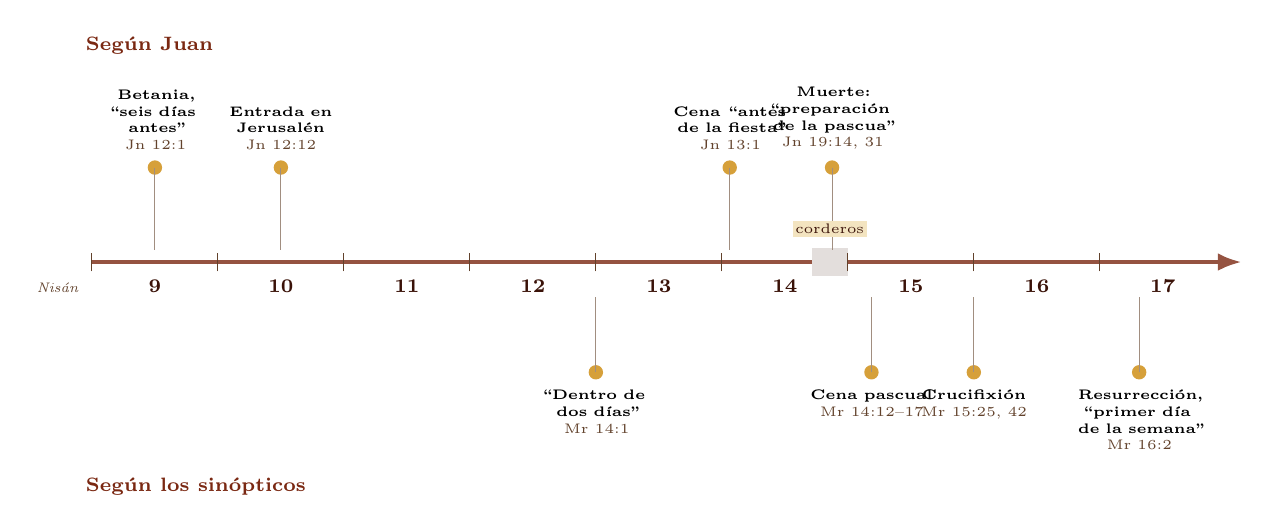
\begin{tikzpicture}[x=1cm,y=1cm,font=\scriptsize]
 \draw[line width=1.4pt,tierraroja!80,-{Latex[length=3mm]}] (0,0) -- (14.6,0);
 \fill[caferojizo!14] (9.15,-0.18) rectangle (9.6,0.18);
 \foreach \x/\d in {0.8/9,2.4/10,4.0/11,5.6/12,7.2/13,8.8/14,10.4/15,12.0/16,13.6/17}{
   \draw[sepia] (\x-0.8,-0.12) -- (\x-0.8,0.12);
   \node[below=3pt,font=\scriptsize\bfseries,text=caferojizo] at (\x,0) {\d};}
 \node[font=\tiny\itshape,text=sepia,anchor=east] at (-0.05,-0.33) {Nisán};
 \node[font=\scriptsize\bfseries,text=tierraroja,anchor=west] at (-0.2,2.75) {Según Juan};
 \foreach \x/\t/\r in {0.8/{Betania, ``seis días antes''}/{Jn 12:1}, 2.4/{Entrada en Jerusalén}/{Jn 12:12}, 8.1/{Cena ``antes de la fiesta''}/{Jn 13:1}, 9.4/{Muerte: ``preparación de la pascua''}/{Jn 19:14, 31}}{
   \fill[mostaza] (\x,1.2) circle (2.6pt);
   \draw[sepia!60] (\x,1.2) -- (\x,0.15);
   \node[above=3pt,text width=1.55cm,align=center,font=\tiny] at (\x,1.2) {\textbf{\t}\\ {\color{sepia}\r}};}
 \node[font=\scriptsize\bfseries,text=tierraroja,anchor=west] at (-0.2,-2.85) {Según los sinópticos};
 \foreach \x/\t/\r in {6.4/{``Dentro de dos días''}/{Mr 14:1}, 9.9/{Cena pascual}/{Mr 14:12--17}, 11.2/{Crucifixión}/{Mr 15:25, 42}, 13.3/{Resurrección, ``primer día de la semana''}/{Mr 16:2}}{
   \fill[mostaza] (\x,-1.4) circle (2.6pt);
   \draw[sepia!60] (\x,-1.4) -- (\x,-0.45);
   \node[below=3pt,text width=1.55cm,align=center,font=\tiny] at (\x,-1.4) {\textbf{\t}\\ {\color{sepia}\r}};}
 \node[font=\tiny,text=caferojizo,fill=papiro,inner sep=1pt] at (9.37,0.42) {corderos};
\end{tikzpicture}\par
{\footnotesize\color{sepia}\textit{Figura 6.} La semana de la Pasión en las dos cronologías (días de Nisán aproximados). \textit{Nota.} Elaboración propia. La asignación de cada hecho a un día concreto es una reconstrucción; las marcas verticales separan los días (de atardecer a atardecer); la franja sombreada marca la tarde del 14, cuando se degollaban los corderos.}
\end{figure}

La diferencia entre Juan y los sinópticos no toca lo que ambos afirman en común: Jesús muere en el tiempo de la Pascua, interpreta su muerte con el pan y la copa de una comida en el marco pascual, y es presentado como la víctima de la Pascua. Los sinópticos lo dicen en la cena y Juan en la hora de la muerte. Esa convergencia es el dato textual sólido; la fecha exacta sigue abierta.


%===================================================================
\section{Lectura literaria}

\subsection{Narración y ley entrelazadas}
Éxodo 12:1--13:16 tiene pocos paralelos en la Torá: el relato se detiene en la noche más dramática para dictar leyes, y las leyes se interrumpen para contar lo que pasó. La instrucción a Moisés (12:1--20) se dicta antes de la plaga; Moisés la transmite a los ancianos (12:21--28); el narrador cuenta la muerte de los primogénitos y la salida (12:29--42); vuelven las normas sobre quién puede comer (12:43--51) y sobre los primogénitos y los Ázimos (13:1--16). El lector vive la noche al mismo tiempo como acontecimiento y como rito, y la forma literaria enseña lo mismo que el contenido: la historia se vuelve liturgia, y la liturgia recuerda la historia.

\begin{figure}[!htbp]\centering
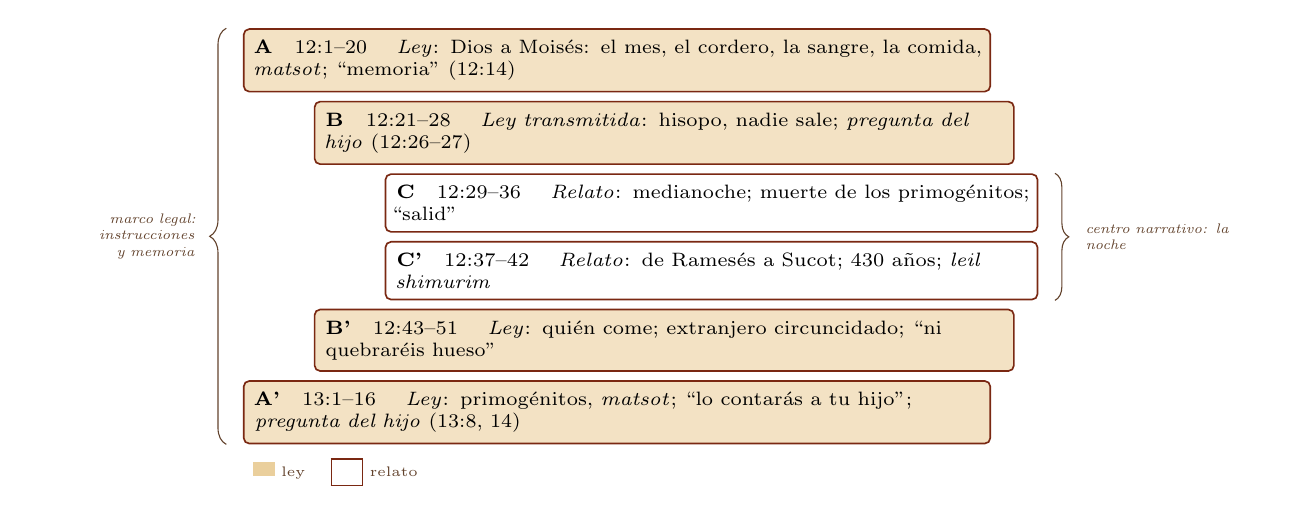
\begin{tikzpicture}[font=\scriptsize,
  bloque/.style={draw=tierraroja,line width=0.6pt,fill=papiro,rounded corners=2pt,text width=9.2cm,align=left,inner sep=4pt,minimum height=0.72cm},
  ley/.style={bloque,fill=mostaza!30},
  relato/.style={bloque,fill=white}]
 \node[ley] (a) at (0,0) {\textbf{A}\quad 12:1--20 \quad \emph{Ley}: Dios a Moisés: el mes, el cordero, la sangre, la comida, \emph{matsot}; ``memoria'' (12:14)};
 \node[ley,below=3pt of a,xshift=0.6cm,text width=8.6cm] (b) {\textbf{B}\quad 12:21--28 \quad \emph{Ley transmitida}: hisopo, nadie sale; \emph{pregunta del hijo} (12:26--27)};
 \node[relato,below=3pt of b,xshift=0.6cm,text width=8.0cm] (c) {\textbf{C}\quad 12:29--36 \quad \emph{Relato}: medianoche; muerte de los primogénitos; ``salid''};
 \node[relato,below=3pt of c,text width=8.0cm] (c2) {\textbf{C'}\quad 12:37--42 \quad \emph{Relato}: de Ramesés a Sucot; 430 años; \emph{leil shimurim}};
 \node[ley,below=3pt of c2,xshift=-0.6cm,text width=8.6cm] (b2) {\textbf{B'}\quad 12:43--51 \quad \emph{Ley}: quién come; extranjero circuncidado; ``ni quebraréis hueso''};
 \node[ley,below=3pt of b2,xshift=-0.6cm] (a2) {\textbf{A'}\quad 13:1--16 \quad \emph{Ley}: primogénitos, \emph{matsot}; ``lo contarás a tu hijo''; \emph{pregunta del hijo} (13:8, 14)};
 \draw[decorate,decoration={brace,amplitude=6pt,mirror},sepia] ([xshift=-6pt]a.north west) -- ([xshift=-6pt]a2.south west) node[midway,left=8pt,text width=2.0cm,align=right,font=\tiny\itshape,text=sepia]{marco legal: instrucciones y memoria};
 \draw[decorate,decoration={brace,amplitude=5pt},sepia] ([xshift=6pt]c.north east) -- ([xshift=6pt]c2.south east) node[midway,right=8pt,text width=2.2cm,align=left,font=\tiny\itshape,text=sepia]{centro narrativo: la noche};
 \node[font=\tiny,text=sepia,anchor=west] at ([yshift=-10pt]a2.south west) {\textcolor{mostaza!50}{\rule{8pt}{5pt}} ley \quad \fcolorbox{tierraroja}{white}{\rule{0pt}{3pt}\hspace{5pt}} relato};
\end{tikzpicture}\par
{\footnotesize\color{sepia}\textit{Figura 7.} Estructura de Éxodo 12:1--13:16 (propuesta). \textit{Nota.} Elaboración propia. La disposición concéntrica es una propuesta de lectura; otros comentarios dividen el texto de otro modo (cf.\ Propp, 1999; Sarna, 1991).}
\end{figure}

\begin{nota}[Precisión]
La estructura de la Figura 7 es una propuesta. Lo que sí está en el texto es la alternancia entre ley y relato, y el lugar de las dos preguntas de los hijos (12:26 y 13:14) en los bloques B y A'. La crítica de fuentes asigna partes de Éxodo 12--13 a distintas tradiciones (sacerdotal, no sacerdotal); esa hipótesis no se discute aquí, porque el estudio lee el texto en su forma final.
\end{nota}

\subsection{De la servidumbre al servicio: \emph{avodá}}
El hilo léxico más fino de Éxodo 12 pasa por la raíz \heb{ע־ב־ד} (\emph{avad}), ``servir, trabajar''. Con ella se describe la opresión de Egipto, ``amargaron su vida con dura servidumbre (\heb{בַּעֲבֹדָה קָשָׁה})'' (Éx 1:14), y con el mismo verbo reclama Dios a Israel: ``deja ir a mi hijo, para que me sirva (\heb{וְיַעַבְדֵנִי})'' (4:23). La Pascua, por su parte, se nombra con el sustantivo:

\hebverso{וּשְׁמַרְתֶּם אֶת־הָעֲבֹדָה הַזֹּאת \\ וְהָיָה כִּי־יֹאמְרוּ אֲלֵיכֶם בְּנֵיכֶם מָה הָעֲבֹדָה הַזֹּאת לָכֶם \\ וַאֲמַרְתֶּם זֶבַח־פֶּסַח הוּא לַיהוָה}
\begin{cita}Y cuando entréis en la tierra que \SENOR{} os dará, como prometió, guardaréis este rito. Y cuando os dijeren vuestros hijos: ¿Qué es este rito vuestro?, vosotros responderéis: Es la víctima de la pascua de \SENOR, el cual pasó por encima de las casas de los hijos de Israel en Egipto, cuando hirió a los egipcios, y libró nuestras casas. Entonces el pueblo se inclinó y adoró.\fuente{(Éx 12:25--27)}\end{cita}

La RVR1960 traduce \emph{avodá} por ``rito'', pero es la misma palabra de la ``servidumbre'' de 1:14. El éxodo no saca a Israel del servicio; le cambia de amo, de la \emph{avodá} de ladrillos a la \emph{avodá} de Dios. El \emph{maror} amargo de 12:8 recuerda la \emph{avodá} amarga de 1:14 (\heb{וַיְמָרְרוּ}), y la \emph{avodá} pascual de 12:25 es la libertad de servir a otro Señor. El juego léxico es explícito en hebreo y se pierde en la traducción.

\subsection{Las preguntas de los hijos}
La Torá prevé cuatro escenas en que un hijo pregunta, o en que el padre debe contar sin que se le pregunte. Tres de ellas pertenecen al relato pascual:

\begin{table}[!htbp]\centering\small\renewcommand{\arraystretch}{1.2}
\begin{tabular}{@{}L{2.0cm}L{5.0cm}L{7.4cm}@{}}
\toprule
\textbf{Texto} & \textbf{Pregunta} & \textbf{Respuesta} \\ \midrule
Éx 12:26--27 & ``¿Qué es este rito vuestro?'' & ``Es la víctima de la pascua de \SENOR, el cual pasó por encima de las casas\ldots{} y libró nuestras casas''. \\
Éx 13:8 & (sin pregunta) & ``Lo contarás en aquel día a tu hijo, diciendo: Se hace esto con motivo de lo que \SENOR{} hizo conmigo cuando me sacó de Egipto''. \\
Éx 13:14 & ``¿Qué es esto?'' & ``\SENOR{} nos sacó con mano fuerte de Egipto, de casa de servidumbre''; de ahí el rescate de los primogénitos. \\
Dt 6:20--25 & ``¿Qué significan los testimonios y estatutos y decretos\ldots?'' & ``Nosotros éramos siervos de Faraón en Egipto, y \SENOR{} nos sacó de Egipto con mano poderosa''; los mandamientos son ``para que nos vaya bien''. \\
\bottomrule
\end{tabular}\par
{\footnotesize\color{sepia}\textit{Tabla 5.} Las preguntas de los hijos. \textit{Nota.} Elaboración propia sobre la RVR1960.}
\end{table}

En las cuatro respuestas el padre no explica un símbolo en abstracto; cuenta una historia en primera persona, plural (``nuestras casas'', ``nos sacó'') o singular (``lo que \SENOR{} hizo \emph{conmigo}'', 13:8), y así cada generación se incluye en el éxodo. La respuesta de 12:27 identifica además el ``rito'' con la ``víctima'': \emph{zevaj-pésaj hu}, ``es sacrificio de pascua''. Sobre esta frase construye la serie su tesis central, que veremos en la sección 7.

\subsection{La Pascua como relato fundante}
El credo histórico de Dt 26:5--9 resume la fe de Israel en una narración: ``Un arameo a punto de perecer fue mi padre, el cual descendió a Egipto\ldots{} y los egipcios nos maltrataron\ldots{} y \SENOR{} nos sacó de Egipto con mano fuerte, con brazo extendido, con grande espanto, y con señales y con milagros; y nos trajo a este lugar, y nos dio esta tierra''. La Pascua es la noche en que esa historia se decide, y por eso los profetas, al anunciar la restauración, la describen como un nuevo éxodo. Isaías llega a invertir el detalle de la prisa: si en Egipto se comió \heb{בְּחִפָּזוֹן} (\emph{bejipazón}), ``apresuradamente'' (Éx 12:11), en el regreso del exilio ``no saldréis apresurados (\heb{לֹא בְחִפָּזוֹן}), ni iréis huyendo; porque \SENOR{} irá delante de vosotros'' (Is 52:12). La alusión es precisa, porque \emph{jipazón} aparece solo en Éx 12:11, Dt 16:3 e Is 52:12 (conteo propio): la segunda salida será más segura que la primera. Jeremías va más lejos y anuncia que el nuevo éxodo eclipsará al antiguo (Jer 16:14--15).

%===================================================================
\section{Memorial, figura y esperanza: la lectura de la serie}

Esta serie tiene un marco propio. Su lectura de la Pascua se resume en cuatro tesis, que expongo aquí con su argumentación y, donde el texto bíblico o la historia lo piden, con precisiones.

\subsection{Reglamento de culto y ley de los ritos}
La serie parte de Hebreos 9:1: ``Ahora bien, aun el primer pacto tenía ordenanzas de culto y un santuario terrenal'', y lee en esa frase dos componentes de la adoración del primer pacto. El \destacar{Reglamento de Culto} son las ``citaciones santas'' de Levítico 23, las solemnidades del \SENOR{} (\heb{מוֹעֲדֵי יְהוָה}, \emph{moadé YHWH}) que Israel debe proclamar como \emph{mikrá kódesh}, ``convocación santa'', ``en sus tiempos'' y por ``estatuto perpetuo''. El \destacar{santuario terrenal}, con su ``ley de los sacrificios'' o ``mandamientos en orden a ritos'' (Ef 2:15, según la Reina-Valera de 1909), son las ofrendas de Números 28--29 y de Levítico 1--7, que daban al hombre un sustituto ante la muerte que merecía su pecado (Ro 6:23).

En mis presentaciones anteriores para la serie añadí dos rasgos a ese marco. El primero es el sentido de \heb{מִקְרָא} (\emph{mikrá}): el término de Lv 23:2 designa una ``convocación'' o ``reunión pública'', y en Neh 8:8 también la ``lectura'' pública de la Ley; allí presenté las solemnidades como \emph{mikrá} en el sentido de ``ensayos'' del plan de Dios. El segundo es la imagen de las fiestas como \destacar{reloj de los tiempos proféticos}: las lumbreras fueron puestas ``por señales y para las estaciones'' (\heb{לְאֹתֹת וּלְמוֹעֲדִים}, Gn 1:14; LXX \grc{εἰς σημεῖα καὶ εἰς καιρούς}), las fiestas son ``sombra de lo por venir'' (Col 2:16--17), y Pablo habla de ``los tiempos y las ocasiones'' (\grc{χρόνων καὶ καιρῶν}, 1~Ts 5:1) y de ``la dispensación del cumplimiento de los tiempos'' (Ef 1:10).

\begin{nota}[Precisión]
``Ensayo'' es una analogía pedagógica, no el significado léxico de \emph{mikrá} (BDB y \emph{HALOT} dan ``convocación, asamblea'' y ``lectura''). Del mismo modo, Gn 1:14 llama \emph{moadim} a los ``tiempos fijados'' por los astros, y el Nuevo Testamento habla de tiempos determinados por Dios; leer en las fiestas un calendario profético es una lectura de la serie que se apoya en esos textos, sin que estos tracen una correspondencia fiesta por fiesta.
\end{nota}

Para la serie, la Pascua es el caso más claro de esa distinción:

\begin{table}[!htbp]\centering\small\renewcommand{\arraystretch}{1.25}
\begin{tabular}{@{}L{6.8cm}L{6.8cm}@{}}
\toprule
\textbf{Reglamento de culto} (Lv 23) & \textbf{Santuario terrenal y ritos} (Éx 12; Nm 28) \\ \midrule
\textbf{Pascua: 14 de Abib} & \textbf{Sacrificio: un cordero} \\
``En el mes primero, a los catorce del mes, entre las dos tardes, pascua es de \SENOR'' (Lv 23:5) & ``Tómese cada uno un cordero\ldots{} y lo inmolará toda la congregación'' (Éx 12:3, 6) \\
Fecha, convocación y memoria: ``este día os será en memoria'' (Éx 12:14) & La víctima: ``Es la víctima de la pascua de \SENOR'' (Éx 12:27) \\
Permanece: la Iglesia la guarda ``hasta que él venga'' (1~Co 11:26) & Se cumple: ``nuestra pascua, que es Cristo, ya fue sacrificada'' (1~Co 5:7) \\
\bottomrule
\end{tabular}\par
{\footnotesize\color{sepia}\textit{Tabla 6.} La Pascua en el esquema de la serie: Reglamento de culto y santuario (He 9:1). \textit{Nota.} Elaboración propia.}
\end{table}

El día 14 de Abib era un día especial para la congregación de Israel según el Reglamento de Culto; pero ese Reglamento nada dice sobre el sacrificio de un cordero, que aparece en Éxodo 12. La prueba principal es la respuesta a los hijos, ``¿Qué es este rito vuestro?\ldots{} Es la víctima de la pascua de \SENOR'' (Éx 12:26--27): el rito de la Pascua era la víctima que se sacrificaba. Esdras 3:4 confirma la distinción: Israel celebró ``la fiesta solemne de los tabernáculos, como está escrito'' (el Reglamento) y ofreció holocaustos ``conforme al rito, cada cosa en su día'' (los sacrificios).

\begin{nota}[Precisión]
(1) En Éx 12:25--26 ``rito'' traduce \heb{עֲבֹדָה} (\emph{avodá}), ``servicio'', y la palabra designa la observancia completa; en 13:5 la misma \emph{avodá} incluye los siete días de \emph{matsot}. La respuesta de 12:27 (\emph{zevaj-pésaj hu}) sí identifica el núcleo de esa \emph{avodá} con la víctima, que es lo que la serie subraya. (2) En Esd 3:4, ``conforme al rito'' traduce \heb{כְּמִשְׁפַּט} (\emph{kemishpat}), ``según la norma''; es otra palabra, aunque el sentido (ofrendas prescritas por día) coincide con la lectura de la serie. (3) Lv 23 no es ajeno a las ofrendas: menciona la ``ofrenda encendida'' de los siete días de Ázimos (23:8) y los sacrificios de las Primicias y de Pentecostés (23:12--13, 18--20), y resume que en cada fiesta se ofrecía ``cada cosa en su tiempo'' (23:37). La distinción de la serie es, por tanto, entre la \emph{fecha y la convocación} (que Lv 23 establece) y el \emph{detalle sacrificial} (que Éx 12 y Nm 28--29 prescriben), no entre un capítulo sin sacrificios y otro con ellos. (4) La autoría de Hebreos es discutida desde la Antigüedad; la serie la atribuye a Pablo, y aquí se respeta esa voz al exponerla.
\end{nota}

\subsection{Memorial de la salvación de los primogénitos}
La primera tesis es histórica. La Pascua queda instituida como memorial de la salvación de Israel de la muerte de los primogénitos en Egipto, con el mandato de celebrarse como estatuto perpetuo. La serie lo apoya en Éx 12:13--14 y en una observación sobre la memoria: un pueblo bajo presión obedece sin preguntar, pero Dios quería que cada momento de la liberación quedara grabado para siempre en la memoria, porque esos hitos históricos simbolizaban el camino que seguirían todos los que oyeran el llamado de Dios. De ahí que la serie lea cada fiesta de Levítico 23 como memorial de un hito de Israel y figura del plan de salvación: la Pascua, la salvación de los primogénitos; Ázimos, la salida de Egipto; el Omer, Israel como primicia de las naciones; Pentecostés, la manifestación del Sinaí.

En el caso de la Pascua, el vínculo entre la fiesta y el hito está en el propio texto, ``Y este día os será en memoria'' (Éx 12:14); no hace falta deducirlo tipológicamente, porque es la razón que la Torá misma da para la fiesta.

\subsection{Tres períodos y una congregación de primogénitos}
La serie ordena la historia de la Iglesia en tres períodos: la Congregación de los Primogénitos (de Adán a Abraham, con una ley tácita transmitida oralmente), Israel como ``la congregación en el desierto'' (Hch 7:38), con el Reglamento de Culto escrito, y la Iglesia del Nuevo Pacto, en la que sus figuras se cumplen en Cristo.

\begin{nota}[Precisión]
La expresión ``congregación de los primogénitos'' viene de He 12:23 (\grc{ἐκκλησίᾳ πρωτοτόκων}), donde designa a la asamblea de la Jerusalén celestial (Lane, 1991; Attridge, 1989); su restricción al período de Adán a Abraham es propia de la serie. El vocabulario es, con todo, pascual: Israel fue el primogénito librado en Egipto (Éx 4:22), y sus primogénitos fueron rescatados la noche de la Pascua (Éx 13:2; Nm 3:13).
\end{nota}

\subsection{Cristo nuestra Pascua}
La segunda tesis es tipológica. La historia del éxodo fue figura simbólica del camino que deberá recorrer la Iglesia. Así como Israel fue esclavo en Egipto y cautivo del faraón, la Iglesia estaba en el Egipto del mundo, presa de Satanás (Ef 2:1--3); así como los hebreos estaban bajo pena de muerte, los gentiles estaban ``muertos en delitos y pecados'' (Ef 2:4--6). Cuando Israel sacrificó la Pascua, quizá no comprendió en ese momento la trascendencia de aquel sencillo acto; pero con la sangre del cordero Dios lo salvó de la muerte, y la sangre de Jesús tiene la misma virtud. La conclusión combina dos textos de Pablo: Cristo es nuestra Pascua, que nos salvó de la muerte (1~Co 5:7; Ef 2:4--5).

\begin{cita}Pero Dios, que es rico en misericordia, por su gran amor con que nos amó, aun estando nosotros muertos en pecados, nos dio vida juntamente con Cristo (por gracia sois salvos).\fuente{(Ef 2:4--5)}\end{cita}

La correspondencia se sostiene en lo que el texto dice expresamente: Pablo identifica a Cristo con \grc{τὸ πάσχα} (1~Co 5:7), y Efesios describe la salvación como paso de la muerte a la vida. Identificar Egipto con el mundo y al faraón con Satanás es ya lectura tipológica de la serie, coherente con el uso paulino del éxodo como ``ejemplo'' para la Iglesia (1~Co 10:1--11), aunque no explícita en esos términos.

\subsection{La Cena: memorial reinstalado ``hasta que él venga''}
La tercera tesis responde a una objeción previsible: si el sacrificio de la Pascua representaba el sacrificio del Hijo de Dios, muerto Jesús, el Cordero de nuestra Pascua, la solemnidad parecería quedar obsoleta; ¿qué valor puede tener ahora su celebración para la Iglesia? La respuesta se busca en la última Pascua de Jesús:

\begin{cita}Porque yo recibí del Señor lo que también os he enseñado: Que el Señor Jesús, la noche que fue entregado, tomó pan; y habiendo dado gracias, lo partió, y dijo: Tomad, comed; esto es mi cuerpo que por vosotros es partido; haced esto en memoria de mí. Asimismo tomó también la copa, después de haber cenado, diciendo: Esta copa es el nuevo pacto en mi sangre; haced esto todas las veces que la bebiereis, en memoria de mí. Así, pues, todas las veces que comiereis este pan, y bebiereis esta copa, la muerte del Señor anunciáis hasta que él venga.\fuente{(1~Co 11:23--26)}\end{cita}

Cumplido el ciclo de la Pascua del primer pacto con la muerte y resurrección de Cristo, Jesús mismo reinstala esta santa solemnidad en el culto como memorial de su sacrificio expiatorio hasta el día en que regrese por su Iglesia. El sacrificio del cordero cesa porque se cumplió, mientras la fecha y el memorial permanecen con nuevos símbolos. La ceremonia incluye el lavamiento de pies (Jn 13:1--15), el pan y el vino como símbolos del cuerpo y la sangre, y se observa una vez al año, al comenzar el día 14 del primer mes.

\begin{nota}[Precisión]
(1) Hay base textual para la continuidad: Jesús vincula el gesto a ``esta pascua'' (Lc 22:15), mira hacia su cumplimiento ``en el reino de Dios'' (22:16) y manda repetirlo (22:19); Pablo lo transmite como tradición recibida (1~Co 11:23) y exhorta: ``celebremos la fiesta'' (\grc{ἑορτάζωμεν}, 1~Co 5:8). (2) La frecuencia es discutida. ``Todas las veces que'' (\grc{ὁσάκις ἐάν}, 1~Co 11:25--26) no fija un intervalo: la serie la entiende como la observancia anual del 14 de Nisán; la mayoría de los intérpretes, como una celebración frecuente, a partir de Hch 2:42, 46 y 20:7. (3) Hubo en el siglo \textsc{ii} cristianos de Asia Menor que celebraban la Pascua el 14 de Nisán, los \emph{cuartodecimanos} (de \emph{quartadecima}, ``decimocuarto''), entre ellos Policarpo de Esmirna, Melitón de Sardes y Polícrates de Éfeso, que apelaban a la tradición del apóstol Juan; Roma la celebraba el domingo (Eusebio, \emph{Historia eclesiástica} 5.23--25). La práctica de la serie tiene, por tanto, un antecedente histórico real, aunque los cuartodecimanos celebraban la Pascua cristiana completa (muerte y resurrección) y no solo la Cena.
\end{nota}

\subsection{El ``rito'' es la víctima}
La cuarta tesis reúne las tres anteriores. Si el ``rito'' de la Pascua era la víctima (Éx 12:27), lo que queda clavado en la cruz (Col 2:14; Ef 2:14--15) son las leyes y ordenanzas de los sacrificios expiatorios (Nm 28--29) y del tratamiento de las impurezas (Lv 12--15), y no el Reglamento de Culto. La Pascua sigue siendo una convocación santa en la que el cordero fue sustituido por el Cordero. Las fiestas son ``sombra de lo que ha de venir'' (Col 2:17), señalan hacia Cristo, y por eso la Iglesia apostólica las siguió guardando (Hch 12:3; 20:6; 1~Co 5:8; 16:8).

\begin{nota}[Precisión]
La lectura de Col 2:16--17 es uno de los puntos más debatidos entre intérpretes. Para la serie, ``nadie os juzgue en cuanto a\ldots{} días de fiesta'' significa que nadie debe juzgar a los creyentes \emph{por guardarlas}, y ``sombra de lo por venir'' indica su valor profético vigente. Para la mayoría de los comentarios, el texto relativiza su observancia porque ``el cuerpo es de Cristo'' (cf.\ Dunn, 1998; Wright, 2013). Ambas lecturas parten del mismo texto griego; la diferencia está en el contexto que cada una reconstruye para la polémica de Colosas. Aquí se expone la de la serie como postura argumentada.
\end{nota}

\begin{figure}[!htbp]\centering
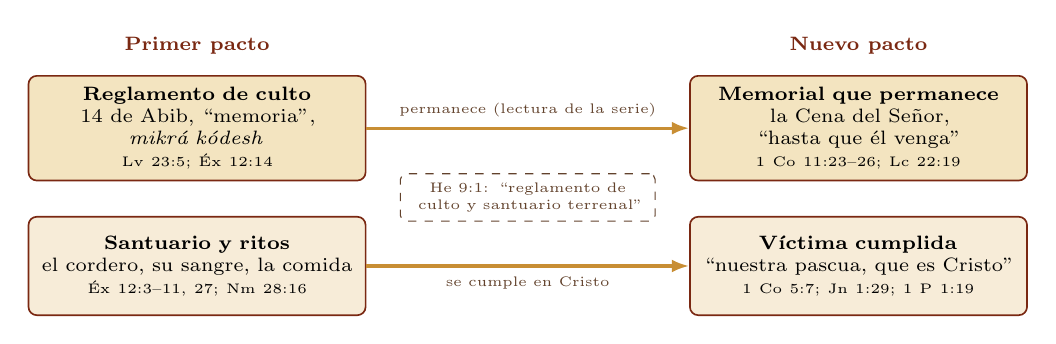
\begin{tikzpicture}[font=\scriptsize,
  col/.style={draw=tierraroja,line width=0.6pt,fill=papiro,rounded corners=3pt,text width=4.0cm,align=center,inner sep=4pt,minimum height=1.25cm},
  fl/.style={-{Latex[length=2.2mm]},mostaza!85!tierraroja,line width=1.1pt}]
 \node[font=\scriptsize\bfseries,text=tierraroja] at (0,1.25) {Primer pacto};
 \node[font=\scriptsize\bfseries,text=tierraroja] at (8.4,1.25) {Nuevo pacto};
 \node[col] (r1) at (0,0.2) {\textbf{Reglamento de culto}\\ 14 de Abib, ``memoria'', \emph{mikrá kódesh}\\ {\tiny Lv 23:5; Éx 12:14}};
 \node[col,fill=mostaza!20] (s1) at (0,-1.55) {\textbf{Santuario y ritos}\\ el cordero, su sangre, la comida\\ {\tiny Éx 12:3--11, 27; Nm 28:16}};
 \node[col] (r2) at (8.4,0.2) {\textbf{Memorial que permanece}\\ la Cena del Señor, ``hasta que él venga''\\ {\tiny 1~Co 11:23--26; Lc 22:19}};
 \node[col,fill=mostaza!20] (s2) at (8.4,-1.55) {\textbf{Víctima cumplida}\\ ``nuestra pascua, que es Cristo''\\ {\tiny 1~Co 5:7; Jn 1:29; 1~P 1:19}};
 \draw[fl] (r1) -- node[above,font=\tiny,text=sepia]{permanece (lectura de la serie)} (r2);
 \draw[fl] (s1) -- node[below,font=\tiny,text=sepia]{se cumple en Cristo} (s2);
 \node[draw=sepia,dashed,rounded corners=2pt,font=\tiny,text=sepia,text width=3.0cm,align=center] at (4.2,-0.68) {He 9:1: ``reglamento de culto y santuario terrenal''};
\end{tikzpicture}\par
{\footnotesize\color{sepia}\textit{Figura 8.} La Pascua en el esquema de la serie. \textit{Nota.} Elaboración propia.}
\end{figure}

%===================================================================
\section{La Pascua en Jesús y los apóstoles}

\subsection{Los evangelios}
Jesús creció en una familia que subía cada año a Jerusalén ``en la fiesta de la pascua'' (Lc 2:41), y Juan ordena el ministerio público en torno a tres Pascuas (Jn 2:13; 6:4; 11:55). La primera enmarca la purificación del templo y el anuncio ``destruid este templo'' (2:19); la segunda, la multiplicación de los panes y el discurso del pan de vida (6:4, 35--58); la tercera, la Pasión. El lector del cuarto evangelio sabe desde el comienzo hacia dónde va el relato, porque el Bautista ya lo ha dicho:

\begin{cita}El siguiente día vio Juan a Jesús que venía a él, y dijo: He aquí el Cordero de Dios, que quita el pecado del mundo.\fuente{(Jn 1:29)}\end{cita}

\grc{Ἴδε ὁ ἀμνὸς τοῦ θεοῦ ὁ αἴρων τὴν ἁμαρτίαν τοῦ κόσμου}. El ``Cordero de Dios'' se ha leído de cuatro maneras: como el cordero pascual (por la cronología de Juan y la cita de 19:36), como el siervo de Isaías 53, que ``como cordero fue llevado al matadero'' y ``llevó el pecado de muchos'' (Is 53:7, 12), como el cordero del sacrificio diario (Éx 29:38--42), o como el carnero victorioso de la apocalíptica judía (Dodd, 1953). Las dos primeras tienen más apoyo en el propio evangelio y no se excluyen (Keener, 2003); la serie sigue la primera.

Los sinópticos sitúan la institución de la Cena en una comida pascual, y Lucas conserva la frase más densa:

\begin{cita}Y les dijo: ¡Cuánto he deseado comer con vosotros esta pascua antes que padezca! Porque os digo que no la comeré más, hasta que se cumpla en el reino de Dios.\fuente{(Lc 22:15--16)}\end{cita}

\begin{cita}Y tomó el pan y dio gracias, y lo partió y les dio, diciendo: Esto es mi cuerpo, que por vosotros es dado; haced esto en memoria de mí. De igual manera, después que hubo cenado, tomó la copa, diciendo: Esta copa es el nuevo pacto en mi sangre, que por vosotros se derrama.\fuente{(Lc 22:19--20)}\end{cita}

Tres rasgos de la cena retoman Éxodo. La \emph{memoria}: ``haced esto en memoria de mí'' (\grc{εἰς τὴν ἐμὴν ἀνάμνησιν}) corresponde al \emph{zikarón} de Éx 12:14. La \emph{sangre del pacto}: ``esto es mi sangre del nuevo pacto'' (Mt 26:28) retoma ``he aquí la sangre del pacto'' de Éx 24:8 y el ``nuevo pacto'' de Jer 31:31. Y el \emph{himno}: ``cuando hubieron cantado el himno, salieron al monte de los Olivos'' (Mt 26:30), que la mayoría de los comentarios identifica con la segunda parte del \emph{Hallel} (Sal 115--118), aunque la Misná que lo prescribe es posterior (m.~Pesajim 10:6--7). También cuenta lo que cambia: Jesús no interpreta el cordero sino el pan y la copa, y el centro de la comida pasa del animal a su propia persona.

Juan, por su parte, acumula detalles pascuales en la cruz. Jesús es condenado ``la preparación de la pascua\ldots{} como la hora sexta'' (19:14); le acercan vinagre ``en un hisopo'' (19:29), la planta con que se pintaron las puertas en Egipto (Éx 12:22); los soldados no le quiebran las piernas, ``para que se cumpliese la Escritura: No será quebrado hueso suyo'' (19:36; véase la sección 5.2). Jesús muere en la hora y con los gestos de la Pascua.

\begin{table}[!htbp]\centering\small\renewcommand{\arraystretch}{1.2}
\begin{tabular}{@{}L{4.0cm}L{2.4cm}L{5.2cm}L{2.6cm}@{}}
\toprule
\textbf{Éxodo 12} & \textbf{Texto} & \textbf{Pasión de Jesús} & \textbf{Texto} \\ \midrule
Se escoge el cordero el día 10 & Éx 12:3 & Entrada en Jerusalén, cinco días antes de la Pascua (lectura tipológica) & Jn 12:1, 12 \\
\emph{Seh tamim}, sin defecto & Éx 12:5 & ``Cordero sin mancha y sin contaminación''; ``Yo no hallo en él ningún delito'' & 1~P 1:19; Jn 18:38 \\
Inmolado ``entre las dos tardes'' del 14 & Éx 12:6 & Muere hacia la hora novena, en la ``preparación de la pascua'' & Mr 15:34--37; Jn 19:14 \\
Sangre en la puerta con hisopo & Éx 12:7, 22 & Esponja con vinagre ``en un hisopo'' & Jn 19:29 \\
``Ni quebraréis hueso suyo'' & Éx 12:46 & ``No será quebrado hueso suyo'' & Jn 19:36 \\
``Este día os será en memoria'' & Éx 12:14 & ``Haced esto en memoria de mí'' & Lc 22:19 \\
``Veré la sangre y pasaré'' & Éx 12:13 & ``Mi sangre del nuevo pacto\ldots{} para remisión de los pecados'' & Mt 26:28 \\
Salida de la servidumbre & Éx 12:41 & ``Rescatados\ldots{} con la sangre preciosa de Cristo'' & 1~P 1:18--19 \\
\bottomrule
\end{tabular}\par
{\footnotesize\color{sepia}\textit{Tabla 7.} Correspondencias entre Éxodo 12 y la Pasión. \textit{Nota.} Elaboración propia. Las correspondencias de las filas 1 y 3 dependen de la cronología joánica y de una lectura tipológica (Chumney, 1994; Baker, 2013); las demás se apoyan en citas o alusiones explícitas.}
\end{table}

\subsection{Pablo: ``nuestra pascua'' y ``el destructor''}
La frase de 1~Co 5:7 aparece en una exhortación moral y no en un tratado sobre el culto. La iglesia de Corinto toleraba un caso de inmoralidad grave, y Pablo responde con el calendario de Pésaj y Matsot:

\begin{cita}Limpiaos, pues, de la vieja levadura, para que seáis nueva masa, sin levadura como sois; porque nuestra pascua, que es Cristo, ya fue sacrificada por nosotros. Así que celebremos la fiesta, no con la vieja levadura, ni con la levadura de malicia y de maldad, sino con panes sin levadura, de sinceridad y de verdad.\fuente{(1~Co 5:7--8)}\end{cita}

El argumento sigue el orden pascual: primero se inmola el cordero (14), después se come sin levadura (15--21). ``Ya fue sacrificada'' (\grc{ἐτύθη}, aoristo) señala un hecho cumplido, y ``celebremos la fiesta'' (\grc{ἑορτάζωμεν}, presente de exhortación), una vida que continúa. Pablo escribe probablemente cerca de la Pascua (cf.\ 16:8, ``estaré en Éfeso hasta Pentecostés''), y la imagen supone que los corintios, en su mayoría gentiles, conocían el ritual (Fee, 1987). La serie ve aquí la prueba de que la Iglesia apostólica guardaba la fiesta, mientras muchos comentaristas leen el pasaje como uso metafórico del calendario. El texto admite ambas cosas, porque Pablo usa la fiesta como imagen precisamente porque la conocen.

En 1~Co 10:1--11 Pablo relee el éxodo como ``ejemplo'' (\grc{τύποι}) para la Iglesia y recuerda a los que ``perecieron por el destructor'' (\grc{ὑπὸ τοῦ ὀλοθρευτοῦ}, 10:10), el agente de la noche pascual; es una advertencia para quienes, ya librados, vuelven a la idolatría.

\subsection{Pedro y Hebreos}
Pedro describe la redención con vocabulario pascual y del éxodo:

\begin{cita}Sabiendo que fuisteis rescatados de vuestra vana manera de vivir, la cual recibisteis de vuestros padres, no con cosas corruptibles, como oro o plata, sino con la sangre preciosa de Cristo, como de un cordero sin mancha y sin contaminación.\fuente{(1~P 1:18--19)}\end{cita}

``Rescatados'' (\grc{ἐλυτρώθητε}) es el verbo con que la LXX describe el éxodo (``os redimiré con brazo extendido'', Éx 6:6) y el rescate de los primogénitos (Éx 13:13), y ``sin mancha'' (\grc{ἄμωμος}) traduce el \emph{tamim} de Éx 12:5. Pedro no dice que Cristo sea el cordero de Pascua en particular, pero redención, sangre y cordero sin defecto, reunidos en una frase, apuntan en esa dirección.

Hebreos 11:28 (de autor discutido) cuenta la Pascua entre los actos de fe de Moisés: ``Por la fe celebró la pascua y la aspersión de la sangre, para que el que destruía a los primogénitos no los tocase a ellos''. Poner la sangre en la puerta fue creer en la palabra de Dios antes de ver el resultado.

\subsection{Apocalipsis: el Cordero como inmolado}
En Apocalipsis 4, Juan contempla el trono de Dios rodeado de veinticuatro ancianos y cuatro seres vivientes que adoran al Creador. En el capítulo 5 aparece un libro sellado que nadie puede abrir, y en ese momento:

\begin{cita}Y miré, y vi que en medio del trono y de los cuatro seres vivientes, y en medio de los ancianos, estaba en pie un Cordero como inmolado, que tenía siete cuernos, y siete ojos, los cuales son los siete espíritus de Dios enviados por toda la tierra.\fuente{(Ap 5:6)}\end{cita}

\begin{cita}Y cantaban un nuevo cántico, diciendo: Digno eres de tomar el libro y de abrir sus sellos; porque tú fuiste inmolado, y con tu sangre nos has redimido para Dios, de todo linaje y lengua y pueblo y nación.\fuente{(Ap 5:9)}\end{cita}

El Cordero está ``en pie'' (\grc{ἑστηκός}), vivo, y a la vez ``como inmolado'' (\grc{ὡς ἐσφαγμένον}), con las marcas de la muerte. Su obra se describe con el lenguaje del éxodo: ``redimido para Dios'' por su sangre, y hecho ``para nuestro Dios reyes y sacerdotes'' (5:10), eco de Éx 19:6. Las plagas de trompetas y copas recuerdan las de Egipto, y los vencedores cantan ``el cántico de Moisés siervo de Dios, y el cántico del Cordero'' (Ap 15:3). La obra de Cristo aparece así como un nuevo éxodo con el Cordero pascual en el centro (Bauckham, 1993), y la adoración del capítulo 4 se extiende a él: ``El Cordero que fue inmolado es digno de tomar el poder, las riquezas, la sabiduría, la fortaleza, la honra, la gloria y la alabanza'' (5:12).

\begin{nota}[Precisión]
La relación tipológica entre la Pascua y la escena del trono de Ap 4--5 es una lectura teológica sostenida por varios intérpretes (el Cordero inmolado, la sangre que redime, el nuevo cántico como cántico del éxodo). El texto de Apocalipsis no menciona la Pascua por nombre; la conexión se apoya en el término \grc{ἀρνίον} \grc{ἐσφαγμένον}, en el vocabulario de redención y en los ecos del éxodo que recorren el libro.
\end{nota}

%===================================================================
\section{La Pascua en la tradición judía}

Después del 70 e.\,c., sin templo y sin cordero, el judaísmo rabínico transformó la Pascua en una comida doméstica de memoria, el \emph{séder} (``orden''), cuya descripción más antigua está en el capítulo 10 de la Misná \emph{Pesajim}. Sus rasgos principales, todos de la tradición posterior, son estos:

\begin{itemize}\setlength{\itemsep}{2pt}
\item \textbf{Cuatro copas} de vino, que ni siquiera el más pobre debe omitir (m.~Pesajim 10:1). Una explicación tradicional las vincula a los cuatro verbos de redención de Éx 6:6--7: ``os sacaré'', ``os libraré'', ``os redimiré'', ``os tomaré'' (Talmud de Jerusalén, Pesajim 10:1).
\item \textbf{Las preguntas del hijo}: ``¿Por qué esta noche es distinta de todas las noches?'' (\emph{Ma nishtaná}, m.~Pesajim 10:4). El padre enseña ``según el entendimiento del hijo'', comenzando ``con la vergüenza'' y terminando ``con la alabanza'', y explica desde ``Un arameo a punto de perecer fue mi padre'' (Dt 26:5) hasta el final del pasaje.
\item \textbf{Las tres cosas de Rabán Gamaliel}: ``Todo el que no dice estas tres cosas en Pascua no ha cumplido su obligación: \emph{pésaj}, \emph{matsá} y \emph{maror}''. Y añade: ``En cada generación el hombre debe verse a sí mismo como si él hubiera salido de Egipto'' (m.~Pesajim 10:5; cf.\ Éx 13:8).

\item \textbf{Los cuatro hijos} de la \emph{Hagadá} (sabio, malvado, simple y el que no sabe preguntar) leen midrásicamente Éx 12:26; 13:8, 14; Dt 6:20 (\emph{Mejilta}).
\item \textbf{El poema de las cuatro noches} del Targum (Neofiti y Pseudo-Jonatán a Éx 12:42) amplía la ``noche de guardar'': la noche de la creación, la de la promesa a Abraham y el sacrificio de Isaac, la de Egipto y la noche futura de la redención mesiánica (Le Déaut, 1963).
\end{itemize}

\begin{nota}[Precisión: lo antiguo y lo reciente en el séder]
Varios elementos que hoy forman parte del \emph{séder} son medievales o modernos: las tres \emph{matsot} sobre la mesa y la mitad escondida como \emph{afikomán} (en la Misná, \emph{afikomán} designa la sobremesa festiva que no debe añadirse después de la Pascua, m.~Pesajim 10:8), la copa de Elías, el huevo y el hueso del plato, y la frase final ``el año próximo en Jerusalén''. Las lecturas cristianas que ven en la \emph{matsá} rayada y perforada, o en la mitad escondida, una figura de la muerte y resurrección de Cristo (p.\,ej.\ Baker, 2013) son aplicaciones devocionales sobre una práctica tardía, no interpretaciones del texto bíblico. La memoria pascual del judaísmo es, con todo, un testimonio de la fuerza de Éx 13:8: cada generación cuenta la salida como propia.
\end{nota}

%===================================================================
\section{Discusión de interpretaciones}

\subsection{Pascua y Cena del Señor}
Que la Cena del Señor nace en el marco de la Pascua lo afirman los cuatro evangelios y Pablo. Qué es esa Cena y cómo se relaciona con la Pascua es lo que divide a los intérpretes:

\begin{table}[!htbp]\centering\small\renewcommand{\arraystretch}{1.2}
\begin{tabular}{@{}L{3.1cm}L{7.6cm}L{3.7cm}@{}}
\toprule
\textbf{Postura} & \textbf{Tesis} & \textbf{Representantes} \\ \midrule
Memorial anual de la Pascua & La Cena es la Pascua del Nuevo Pacto; se celebra una vez al año, el 14 de Nisán, con pan, vino y lavamiento de pies; el cordero se cumplió en Cristo & Serie; antecedente: cuartodecimanos \\
Memorial (conmemoración) & La Cena recuerda la muerte de Cristo y la proclama; los elementos son signos & Zuinglio \\
Presencia espiritual & Cristo se da realmente al creyente por el Espíritu en la Cena & Calvino \\
Cumplimiento escatológico & La ``memoria'' mira hacia adelante: pide a Dios que recuerde al Mesías y traiga el reino (``hasta que él venga'') & Jeremias (1966) \\
\bottomrule
\end{tabular}\par
{\footnotesize\color{sepia}\textit{Tabla 8.} Posturas sobre la relación entre la Pascua y la Cena del Señor. \textit{Nota.} Elaboración propia.}
\end{table}

Dos datos textuales pesan en este debate. La \grc{ἀνάμνησις} recoge el horizonte del \emph{zikarón}, una memoria que actualiza el acontecimiento para cada generación (Éx 13:8, ``lo que \SENOR{} hizo \emph{conmigo}''), y la Cena mira también hacia adelante, ``hasta que se cumpla en el reino de Dios'' (Lc 22:16), ``hasta que él venga'' (1~Co 11:26). En esto coinciden la serie y Jeremias; difieren en la frecuencia y la forma de la observancia.

\subsection{¿Era el cordero pascual un sacrificio expiatorio?}
La serie llama a la Cena memorial del sacrificio expiatorio de Cristo, y en general lee el cordero pascual como figura de la expiación de Cristo. La pregunta tiene un lado exegético preciso: qué clase de sacrificio era la Pascua en la Torá.

\textbf{Argumentos para una lectura no expiatoria.} Éxodo 12 llama a la Pascua \heb{זֶבַח} (\emph{zevaj}, sacrificio que se come) y no \heb{חַטָּאת} (\emph{jatat}, ``por el pecado''); la familia come toda la carne; la sangre va a la puerta y no a un altar, como señal protectora (``apotropaica''); y el capítulo no menciona pecado ni perdón (Propp, 1999; Sarna, 1991). La Pascua salvaría de la muerte más que del pecado.

\textbf{Argumentos para una lectura expiatoria o sustitutiva.} El primogénito israelita no se salva por mérito ni por etnia, sino por una muerte en su lugar: donde hay sangre no muere el hijo. La Torá posterior funda en la sangre la expiación (Lv 17:11), y en el Segundo Templo la sangre pascual se rociaba en el altar (2~Cr 35:11; m.~Pesajim 5:6). Ezequiel asocia un \emph{jatat} al día 14 (Ez 45:22). Y el Nuevo Testamento une el lenguaje pascual con el del pecado: el Cordero ``quita el pecado del mundo'' (Jn 1:29), la sangre de la copa es ``para remisión de los pecados'' (Mt 26:28), y Pedro habla de rescate por la sangre del cordero sin mancha (1~P 1:18--19).

\begin{nota}[Precisión: una síntesis posible]
Las dos lecturas no se contradicen si se distinguen los niveles. En Éxodo 12, la Pascua es un sacrificio de comunión cuya sangre protege de la muerte por sustitución; no es un \emph{jatat}. En la lectura del Nuevo Testamento, Cristo cumple a la vez la Pascua (liberación de la muerte y del dominio ajeno), el sacrificio del pacto (Éx 24:8) y la expiación por el pecado (Is 53; Lv 16); los autores combinan esas figuras sin confundirlas (Dunn, 1998; Wright, 2013). Llamar a la Pascua ``expiatoria'' es correcto como lectura cristológica integrada; como descripción del rito de Éxodo 12 requiere esa precisión. La propia serie lo insinúa al hablar de la Pascua como salvación ``de la muerte'' (Ef 2:4--5).
\end{nota}

%===================================================================
\section{Síntesis}

\begin{tcolorbox}[enhanced,unbreakable,colback=papiro,colframe=tierraroja,boxrule=1pt,arc=3pt,title={Pésaj, la Pascua del \SENOR},fonttitle=\bfseries,colbacktitle=tierraroja,coltitle=papiro]
La Pascua es la solemnidad del 14 de Abib, ``entre las dos tardes'' (Lv 23:5), \destacar{memorial perpetuo} (Éx 12:14) de la noche en que el \SENOR{} juzgó a Egipto, \destacar{vio la sangre} y \destacar{pasó por encima} de las casas de Israel, librando a sus primogénitos (Éx 12:12--13, 27): vida recibida por una muerte sustituta, contada por cada generación como propia (Éx 13:8). El Nuevo Testamento la ve cumplida en Jesús, ``nuestra pascua'' (1~Co 5:7), cuyo memorial se celebra ``hasta que él venga'' (1~Co 11:26) y a quien, como Cordero inmolado, adoran los redimidos (Ap 5:9--12).
\end{tcolorbox}

\begin{table}[!htbp]\centering\small\renewcommand{\arraystretch}{1.22}
\begin{tabular}{@{}L{3.0cm}L{11.4cm}@{}}
\toprule
\textbf{Lectura} & \textbf{Aporte a la comprensión de la Pascua} \\ \midrule
Histórica & La fiesta pertenece al mes de las espigas y a la luna llena; nace en el delta oriental de Egipto como juicio sobre el faraón y sus dioses; la historia de Israel la renueva en cada fundación (Gilgal, Ezequías, Josías, Esdras); en el Segundo Templo es la gran peregrinación. \\
Filológica & \emph{Pésaj} une ``pasar por encima'' y ``proteger''; \emph{ot} hace de la sangre una señal ``para vosotros''; \emph{maror} y \emph{avodá} conectan la comida con la servidumbre; \grc{πάσχα} pasa intacta de la LXX a Pablo. \\
Textual & Los 430 años (TM, LXX, PS y Gá 3:17); el ``hervir'' de Dt 16:7 armonizado en 2~Cr 35:13; Jn 19:36 combina Éx 12:46 y Sal 34:20; la fecha de la cena queda abierta. \\
Literaria & Éxodo 12--13 entrelaza ley y relato; las preguntas de los hijos convierten la historia en catequesis; la \emph{avodá} de ladrillos se vuelve \emph{avodá} de Dios; Isaías invierte la prisa del primer éxodo. \\
La serie & Memorial de la salvación de los primogénitos; el ``rito'' es la víctima; el cordero se cumple en Cristo y el memorial permanece en la Cena, ``hasta que él venga''. \\
Nuevo Testamento & Cordero de Dios, sangre del nuevo pacto, rescate por sangre, Cordero inmolado en el trono: la Pascua es clave de lectura de la cruz. \\
\bottomrule
\end{tabular}\par
{\footnotesize\color{sepia}\textit{Tabla 9.} Lectura y aporte. \textit{Nota.} Elaboración propia.}
\end{table}

%===================================================================
\section{Para la reflexión}

\begin{enumerate}\setlength{\itemsep}{3pt}
\item En Egipto, la sangre debía estar en la puerta \emph{antes} de la medianoche, y la familia debía quedarse dentro ``hasta la mañana'' (Éx 12:22). ¿Qué significa, en concreto, permanecer ``dentro de la casa'' marcada por la sangre de Cristo, y no solo haberla marcado una vez?
\item La sangre fue señal ``para vosotros'' (Éx 12:13). ¿En qué descansa la seguridad del creyente: en lo que Dios ve o en lo que uno siente? Hebreos 11:28 dice que Moisés celebró la Pascua ``por la fe'', antes de ver el resultado.
\item ``Lo contarás en aquel día a tu hijo'' (Éx 13:8). ¿Cómo se responde, con la propia historia y no solo con doctrina, cuando un hijo, un alumno o un hermano pregunta ``¿qué es este rito vuestro?''
\item Pablo une la Pascua con la limpieza de la levadura (1~Co 5:7--8). Antes de participar del memorial, ¿qué ``levadura de malicia y de maldad'' hay que quitar de la casa?
\end{enumerate}

%===================================================================
\section*{Glosario}\markboth{Glosario}{}
\begin{description}\setlength{\itemsep}{2pt}
\item[Abib] (\heb{אָבִיב}). ``Espiga verde'' de cebada; nombre del primer mes en la Torá (Éx 13:4), luego Nisán.
\item[\emph{Avodá}] (\heb{עֲבֹדָה}). ``Servicio, trabajo''; la ``servidumbre'' de Egipto (Éx 1:14) y el ``rito'' de la Pascua (Éx 12:25--26).
\item[\emph{Bein ha'arbayim}] (\heb{בֵּין הָעַרְבָּיִם}). ``Entre las dos tardes''; hora del sacrificio pascual (Éx 12:6; Lv 23:5).
\item[\emph{Maror}] (\heb{מָרוֹר}). ``Hierba amarga'' (Éx 12:8), de la raíz de ``amargaron'' (Éx 1:14).
\item[\emph{Mashjit}] (\heb{מַשְׁחִית}). ``Destructor''; agente del juicio que no entra en las casas marcadas (Éx 12:23).
\item[\emph{Mezuzot} y \emph{mashqof}] (\heb{מְזוּזֹת}, \heb{מַשְׁקוֹף}). ``Postes'' y ``dintel'' de la puerta (Éx 12:7, 22--23; Dt 6:9).
\item[\emph{Pascha}] (\grc{πάσχα}). Transcripción griega del arameo \emph{pasja}; fiesta, cordero y comida.
\item[\emph{Pésaj}] (\heb{פֶּסַח}). ``Pascua''; de \emph{p-s-j}, ``pasar por encima, proteger''.
\item[\emph{Seh tamim}] (\heb{שֶׂה תָמִים}). ``Res menor sin defecto'', oveja o cabra (Éx 12:5).
\item[\emph{Zevaj}] (\heb{זֶבַח}). ``Sacrificio'' que se come; ``víctima de la pascua'' (Éx 12:27).
\item[\emph{Zikarón}] (\heb{זִכָּרוֹן}). ``Memoria, memorial'' (Éx 12:14); en griego \grc{ἀνάμνησις} (Lc 22:19).
\end{description}

%===================================================================
\section*{Referencias}\markboth{Referencias}{}
\refapa{Attridge, H.~W. (1989). \emph{The epistle to the Hebrews} (Hermeneia). Fortress Press.}
\refapa{Baker, D. (2013). \emph{El poder espiritual de las siete fiestas de Dios}. Editorial Imagen.}
\refapa{Bauckham, R. (1993). \emph{The climax of prophecy: Studies on the book of Revelation}. T\&T Clark.}
\refapa{Bokser, B.~M. (1984). \emph{The origins of the Seder: The Passover rite and early rabbinic Judaism}. University of California Press.}
\refapa{Brown, F., Driver, S.~R., \& Briggs, C.~A. (1906). \emph{A Hebrew and English lexicon of the Old Testament}. Clarendon Press.}
\refapa{Brown, R.~E. (1994). \emph{The death of the Messiah: From Gethsemane to the grave} (2 vols.). Doubleday.}
\refapa{Chumney, E. (1994). \emph{The seven festivals of the Messiah}. Destiny Image.}
\refapa{Danby, H. (Trad.). (1933). \emph{The Mishnah}. Oxford University Press.}
\refapa{Dodd, C.~H. (1953). \emph{The interpretation of the Fourth Gospel}. Cambridge University Press.}
\refapa{Dunn, J.~D.~G. (1998). \emph{The theology of Paul the apostle}. Eerdmans.}
\refapa{Elliger, K., \& Rudolph, W. (Eds.). (1997). \emph{Biblia Hebraica Stuttgartensia} (5.ª ed.). Deutsche Bibelgesellschaft.}
\refapa{Eusebio de Cesarea. (1973). \emph{Historia eclesiástica} (A. Velasco-Delgado, Trad.; 2 vols.). Biblioteca de Autores Cristianos.}
\refapa{Fee, G.~D. (1987). \emph{The first epistle to the Corinthians} (NICNT). Eerdmans.}
\refapa{Hall, S.~G. (Ed. y Trad.). (1979). \emph{Melito of Sardis: On Pascha and fragments}. Clarendon Press.}
\refapa{Hoffmeier, J.~K. (1997). \emph{Israel in Egypt}. Oxford University Press.}
\refapa{Humphreys, C.~J. (2011). \emph{The mystery of the Last Supper}. Cambridge University Press.}
\refapa{Jaubert, A. (1957). \emph{La date de la Cène: Calendrier biblique et liturgie chrétienne}. Gabalda.}
\refapa{Jeremias, J. (1966). \emph{The eucharistic words of Jesus} (N. Perrin, Trad.). SCM Press.}
\refapa{Josefo, F. (1997). \emph{Antigüedades judías} (J. Vara Donado, Trad.). Akal.}
\refapa{Josefo, F. (1999). \emph{La guerra de los judíos: Libros IV--VII} (J.~M. Nieto Ibáñez, Trad.). Gredos.}
\refapa{Keener, C.~S. (2003). \emph{The Gospel of John: A commentary} (2 vols.). Hendrickson.}
\refapa{Koehler, L., \& Baumgartner, W. (2001). \emph{The Hebrew and Aramaic lexicon of the Old Testament} (2 vols.). Brill.}
\refapa{Lane, W.~L. (1991). \emph{Hebrews 9--13} (WBC 47B). Word Books.}
\refapa{Le Déaut, R. (1963). \emph{La nuit pascale}. Institut Biblique Pontifical.}
\refapa{Meier, J.~P. (1991). \emph{A marginal Jew: Rethinking the historical Jesus} (Vol. 1). Doubleday.}
\refapa{Nestle, E., \& Aland, K. (Eds.). (2012). \emph{Novum Testamentum Graece} (28.ª ed.). Deutsche Bibelgesellschaft.}
\refapa{Porten, B., \& Yardeni, A. (1986). \emph{Textbook of Aramaic documents from ancient Egypt: Vol. 1. Letters}. Hebrew University.}
\refapa{Propp, W.~H.~C. (1999). \emph{Exodus 1--18} (Anchor Bible 2). Doubleday.}
\refapa{Rahlfs, A., \& Hanhart, R. (Eds.). (2006). \emph{Septuaginta} (ed. rev.). Deutsche Bibelgesellschaft.}
\refapa{Sarna, N.~M. (1991). \emph{Exodus} (JPS Torah Commentary). Jewish Publication Society.}
\refapa{Sefaria. (s.~f.). \emph{Mishnah Pesachim; Rashi on Exodus; Targum Onkelos}. https://www.sefaria.org}
\refapa{Sociedades Bíblicas en América Latina. (1960). \emph{Santa Biblia: Reina-Valera 1960}.}
\refapa{Tigay, J.~H. (1996). \emph{Deuteronomy} (JPS Torah Commentary). Jewish Publication Society.}
\refapa{VanderKam, J.~C. (1998). \emph{Calendars in the Dead Sea Scrolls: Measuring time}. Routledge.}
\refapa{Wright, N.~T. (2013). \emph{Paul and the faithfulness of God} (2 vols.). Fortress Press.}

\end{document}
